% !TEX encoding = UTF-8
% !TEX TS-program = pdflatex
% !TEX root = ../tesi.tex


\chapter{Simulations}
	\label{chapter:simulations}
	After the protocols under consideration have been presented in Chapters \ref{chapter:fb} and \ref{chapter:roff}, this Chapter will contain the results of the simulation carried out through various scenarios of increasing complexity. Several algorithms will be tested, namely:
	\begin{itemize}
		\item Fast-Broadcast and SJ-Fast-Broadcast;
		\item ROFF and SJ-ROFF;
		\item STATIC variants of Fast-Broadcast (e.g. STATIC-100), which behave like Fast-Broadcast but do not employ a transmission range estimation. They only use a static parameter (for example 100 meters for STATIC-100) and use it in the Broadcast Phase;
		\item SJ-STATIC variants of Fast-Broadcast, which also considers junctions during message propagation, but do not employ a transmission range estimation.
	\end{itemize}
	
	
	Numeric results in every chart will be coupled with their 95\% confidence interval. All following simulation have been run on the High Performance Computing platform of the University of Padua, Department of Mathematics \cite{cluster}.
	
	\section{Metrics}
		\label{sec:metrics}
		Before proceeding with the presentation of simulation results, the metrics used to evaluate the protocols' performances will be presented in this section. 
		
		\subsection{Total Delivery Ratio (TDR)}
			\label{ssec:tdr}
			This metric is used to detect how many vehicles have received the Alert Message in total. Ideally, broadcasting protocols should be able to reach all the reachable nodes in the scenario in order to warn them of the danger. The metric is calculated as follows:
			
			\begin{gather}
				\label{eq:tdr}
				\textit{TDR} = \frac{\textrm{\textit{no. of vehicles successfully receiving the Alert Message}}}{\textrm{\textit{no. of vehicles in the scenario}}}
			\end{gather}
			
			All scenarios are created in a way such that every node can be reached by multi-hop propagation regardless of the source of the Alert Message. In other words, from graph theory point of view, the graph resulting from vehicle distribution where two nodes are connected only if they are within transmission range of each other is a connected graph. This way, the term at the denominator of Equation \ref{eq:tdr} is equivalent to the number of vehicles reachable by pure flooding.
			
		\subsection{Total Delivery Ratio On Circumference (TDROC)}
			This metric is used to detect how many vehicles on the circumference (i.e. the area of interest where the alert data has to be delivered) have received the Alert Message. The circumference is built starting from the source of the Alert Message. The way it is built depends on scenario topology (e.g. 1D, 2D, etc) and will be explained more thoroughly in the following sections. Basically, this metric considers only vehicles far from the source of the AM, instead of all vehicles as in the previous metric. Hence, this is used to measure how effective the algorithm is at delivering the message far from the origin. The metric is calculated as follows:
			
			\begin{gather}
			 	\label{eq:tdroc}
			 	\textit{TDROC} = \frac{\textrm{\textit{no. of vehicles on circ. successfully receiving the Alert Message}}}{\textrm{\textit{no. of vehicles on circ.}}}
			\end{gather}
		
			The same consideration about vehicles and reachability by pure flooding presented in Section \ref{ssec:tdr} is also valid for Equation \ref{eq:tdroc}.
			
		\subsection{Number Of Hops (NOH)}
			This metric is used to measure the mean number of hops required in order to propagate the Alert Message from the source to all vehicles reached on the circumference. This value is obviously dependent on the paths taken by forwarded Alert Messages from the source to all destinations. We have that \textit{NOH} is always greater than or equal to the \textit{Optimal Number of Hops ONOH} (i.e. $ONOH \leq NOH$). \textit{ONOH} is calculated using the following formula:
			$$ ONOH = \frac{\textrm{\textit{Circumference Radius}}}{\textrm{\textit{Transmission Range}}} $$
			
			The Number Of Hops metric can be calculated as follows:
			
			\begin{gather}
				\label{eq:noh}
				\textit{NOH} = \frac{ \sum_{p \in RC } \textrm{\textit{no. of hops from source to p}}} {\textrm{|\textit{RC}|}}
			\end{gather}
			
			where $RC$ is the set of vehicles which have successfully received the message on the circumference.
			
			
			The \textit{NOH} metric (whose value should be as close as possible to \textit{ONOH}) is an important indicator of the effectiveness of the multi-hop protocol in choosing the farthest forwarder during contention.
			
			
			Figure \ref{fig:hops} can be used as an example to calculate \textit{NOH}. Using Equation \ref{eq:noh}, the mean number of hops is equal to 3.
			
			\begin{figure}[H]
				\centering
				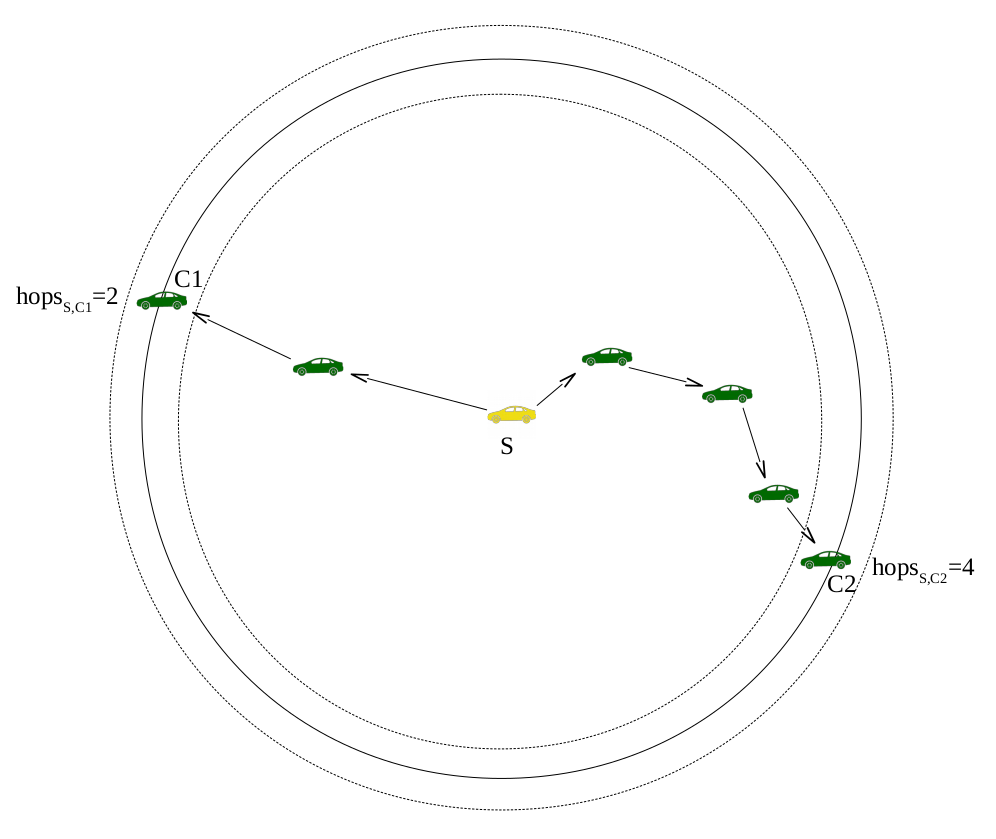
\includegraphics[width=0.7\textwidth]{immagini/hops}
				\caption{Example of \textit{NOH} calculation with Alert Message starting from node S}
				\label{fig:hops}
			\end{figure}
			
		\subsection{Number Of Slots (NOS)}
			This metric is used to measure the number of slots required in order to propagate the Alert Message from the source to all vehicles reached on the circumference. High values of this metric means that the multi-hop protocol introduces a lot of waiting time before each forwarding, hence increasing end-to-end delay and hurting the timeliness of the emergency message propagation.
		
			\begin{gather}
				\label{eq:slots}
				\textit{NOS} = \frac{ \sum_{p \in RC } \textrm{\textit{no. of slots waited along path from source to p}}}  {\textrm{|\textit{RC}|}}
			\end{gather}	
	
			where $RC$ is the set of vehicles which have successfully received the message on the circumference.
			The number of slots along the path from node $a$ to $b$ at the numerator of Equation \ref{eq:slots} is the sum of the slots waited by each forwarder before relaying the Alert Message. 
			
			
			Based on the scenario represented in Figure \ref{fig:slots} and Equation \ref{eq:slots}, the mean number of slots from source S to nodes on the circumference is 100.
			
			\begin{figure}[H]
				\centering
				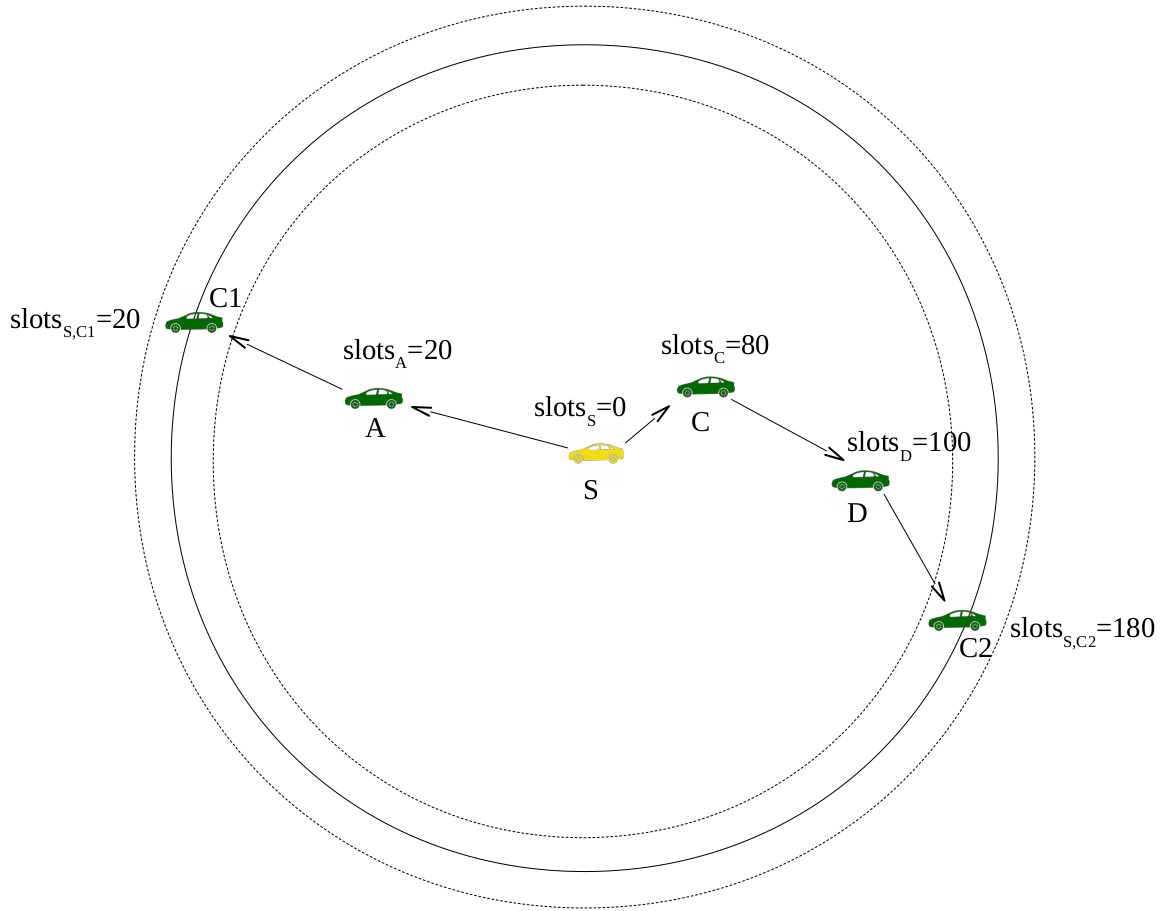
\includegraphics[width=0.7\textwidth]{immagini/slots}
				\caption{Example of \textit{NOS} calculation with Alert Message starting from node S}
				\label{fig:slots}
			\end{figure}
			
			
		\subsection{Forwarding Node Number (FNN)}
			This metric is used to measure the number of vehicles which forward the Alert Message. The value of this metric is an indicator of the effectiveness of the multi-hop protocol in successfully suppressing scheduled transmissions from \acrshort{pfca}s after the \acrshort{ffca} has relayed the message. The metric is calculated as follows:
			 
			\begin{gather}
				\label{eq:nos}
				\textit{FNN} = \textrm{\textit{no. of vehicles forwarding the Alert Message}}
			\end{gather}	
				
	\section{Platoon scenario}
		The first scenario taken into consideration is a simple one-dimensional platoon scenario, where vehicles are placed in a strip-like area 15 kilometers long. Vehicles are 25 meters distant from each other. Transmission ranges of 100, 300 and 500 meters has been employed during simulations. 
		Parameters for this scenario are included in Table \ref{table:platoon}.  These parameters will also be valid for all following scenarios, unless specified otherwise.
		
		\begin{table}[H]
			\def\arraystretch{1.1}
			\rowcolors{2}{D}{P}	
			\begin{tabularx}{\textwidth}{l | l  l}
				\rowcolor{I} {\large \textcolor{white}{Parameter}} & {\large \textcolor{white}{Value}} & {\large \textcolor{white}{}} \TBstrut  \\
				\toprule
				\endhead
	%			\midrule[1pt]
				\rowcolor{P} \multicolumn{3}{c}{Scenario configuration} \\
				\midrule[1pt]
				Road length 							& 15000 				& m		\\
				Distance between vehicles 				& 25					& m		\\
				Circumference	radius					& 14000					& m		\\
				Number of vehicles						& 600					& 		\\
				Source of alert message position		& Left of platoon		&		\\
				\midrule[1pt]
				\rowcolor{P} \multicolumn{3}{c}{Network configuration} \\
				\midrule[1pt]
				Packet payload size						& 100					& byte	\\	
				Transmission standard					& 802.11b				&		\\
				Frequency								& 2.4					& GHz	\\
				Channel bandwidth						& 22					& MHz	\\
				Transmission speed						& 11					& Mbps	\\
				Transmission powers						& -7.0, 4.6, 13.4		& dBm	\\
				Transmission range						& 100, 300, 500			& m		\\
				Modulation								& DSSS					& 		\\
				Mobility model							& ns3::ConstantPosition	&		\\
				Propagation loss model					& ns3::TwoRayGround 	&		\\
				Propagation delay model					& ns3::ConstantSpeed	&		\\
				Shadowing model							& No					&		\\
				Junction modeling						& No					&		\\
				\midrule[1pt]
				\rowcolor{P} \multicolumn{3}{c}{Protocols configuration} \\
				\midrule[1pt]
	%			Protocols tested						& \makecell{FB, ROFF, STATIC100, \\ STATIC300, STATIC500} & \\
				FB contention window					& [32, 1024]			& slot	\\
				ROFF distance range (\textit{k} parameter) & 1					&		\\	
				\midrule[1pt]
				Number of simulations per configuration	& 1000					&		\\
				\bottomrule
			\end{tabularx}
			\caption{Platoon scenario configuration}
			\label{table:platoon}
		\end{table}
	
		\begin{figure}[H]
			\centering
			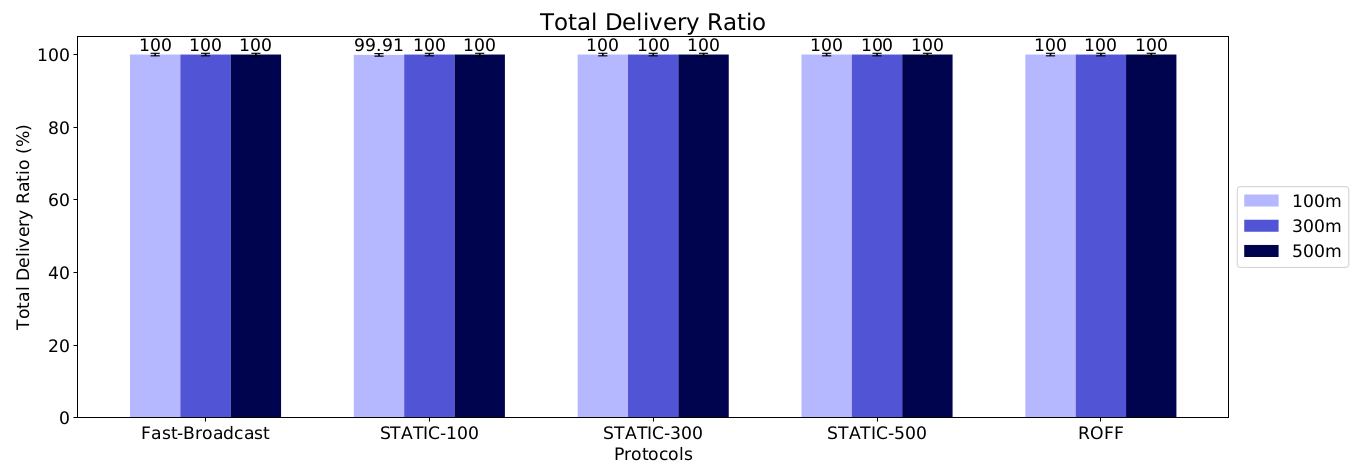
\includegraphics[width=1.1\textwidth]{immagini/platoon-15km/tdr}
			\caption{\textit{TDR} metric for Platoon scenario}
			\label{fig:metric-platoon-15km-0}
		\end{figure}
	
		\begin{figure}[H]
			\centering
			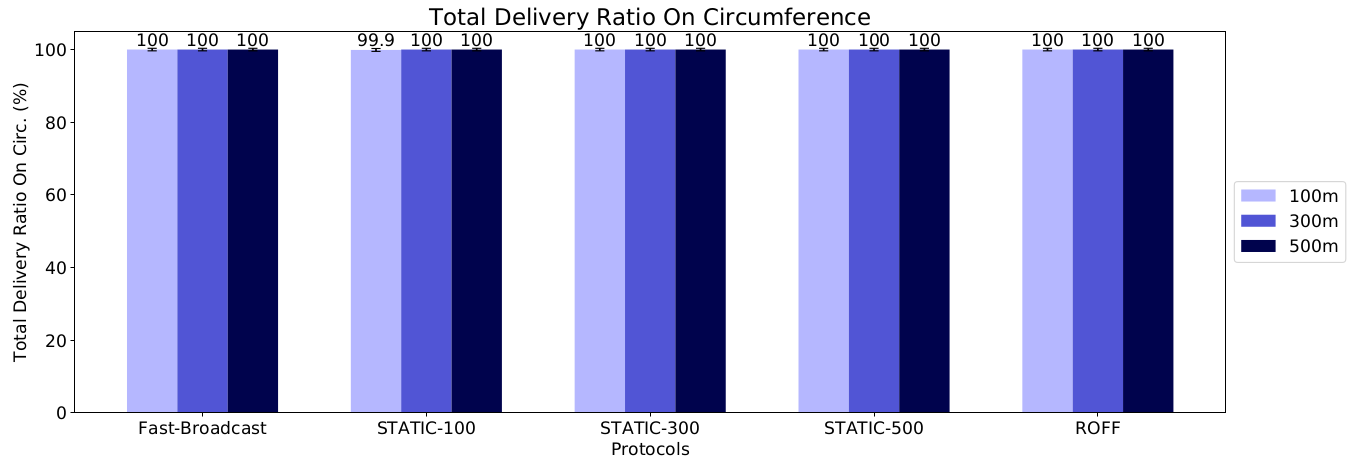
\includegraphics[width=1.1\textwidth]{immagini/platoon-15km/tdroc}
			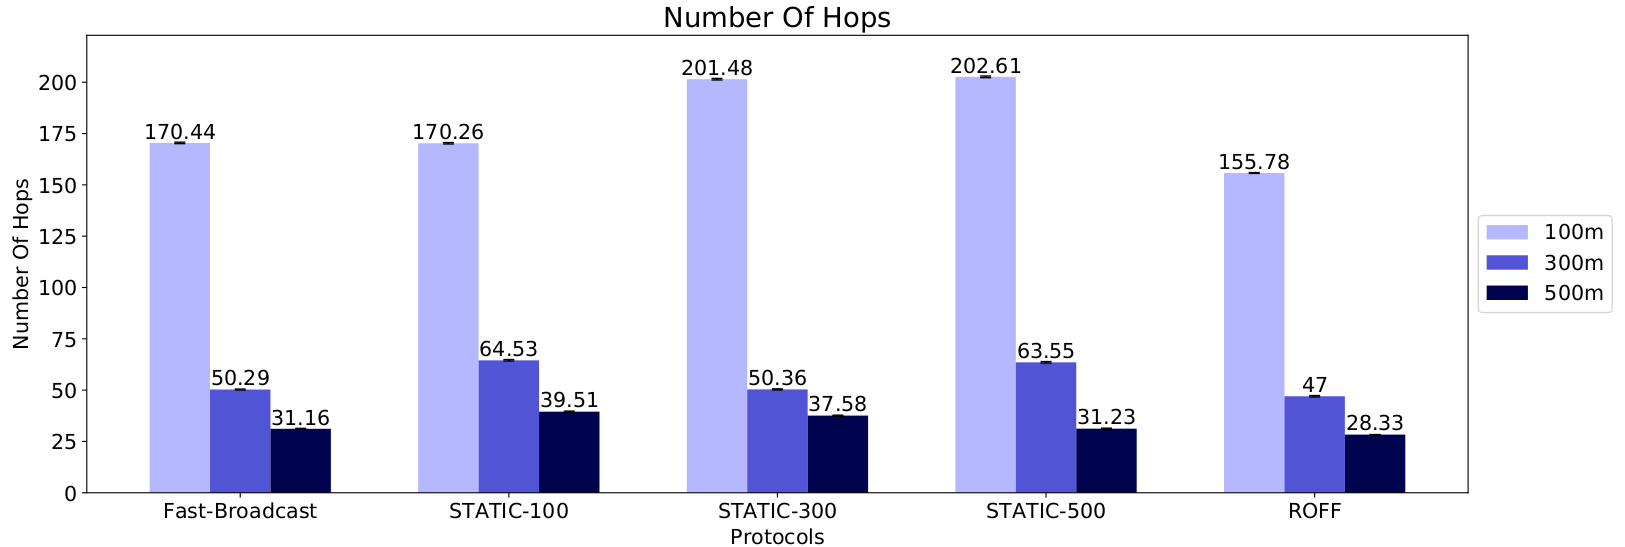
\includegraphics[width=1.1\textwidth]{immagini/platoon-15km/noh}
			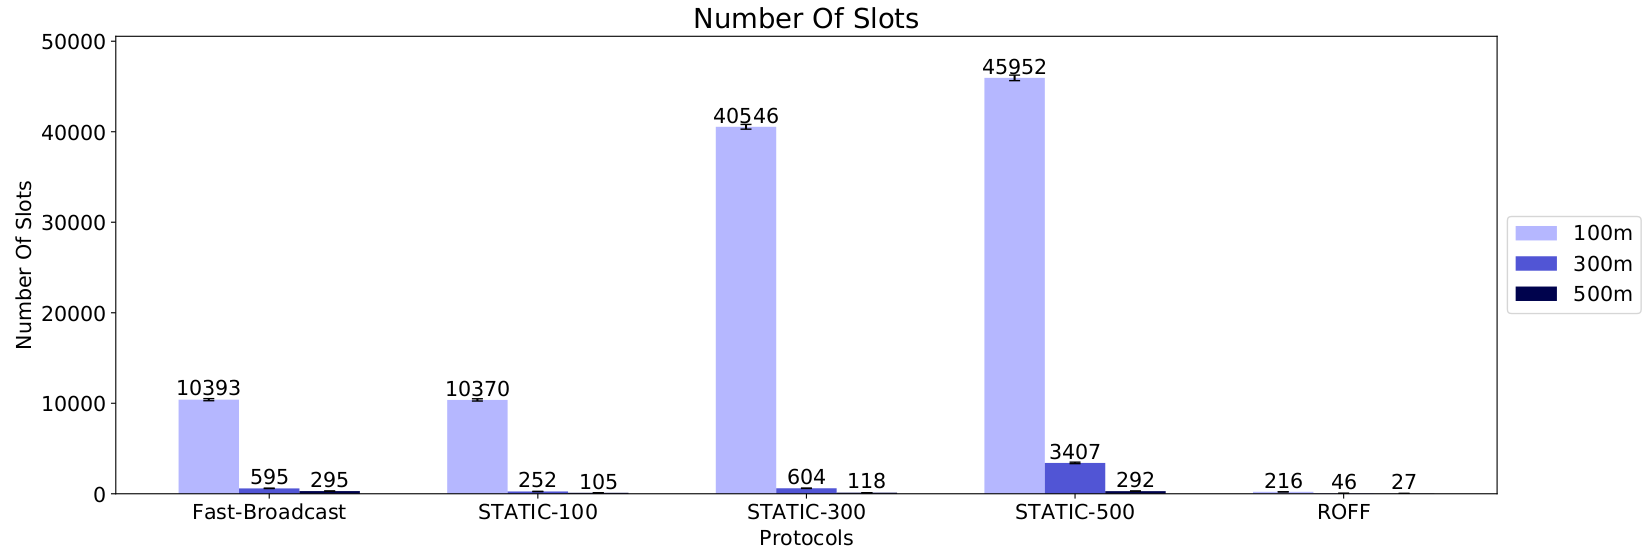
\includegraphics[width=1.1\textwidth]{immagini/platoon-15km/nos}
			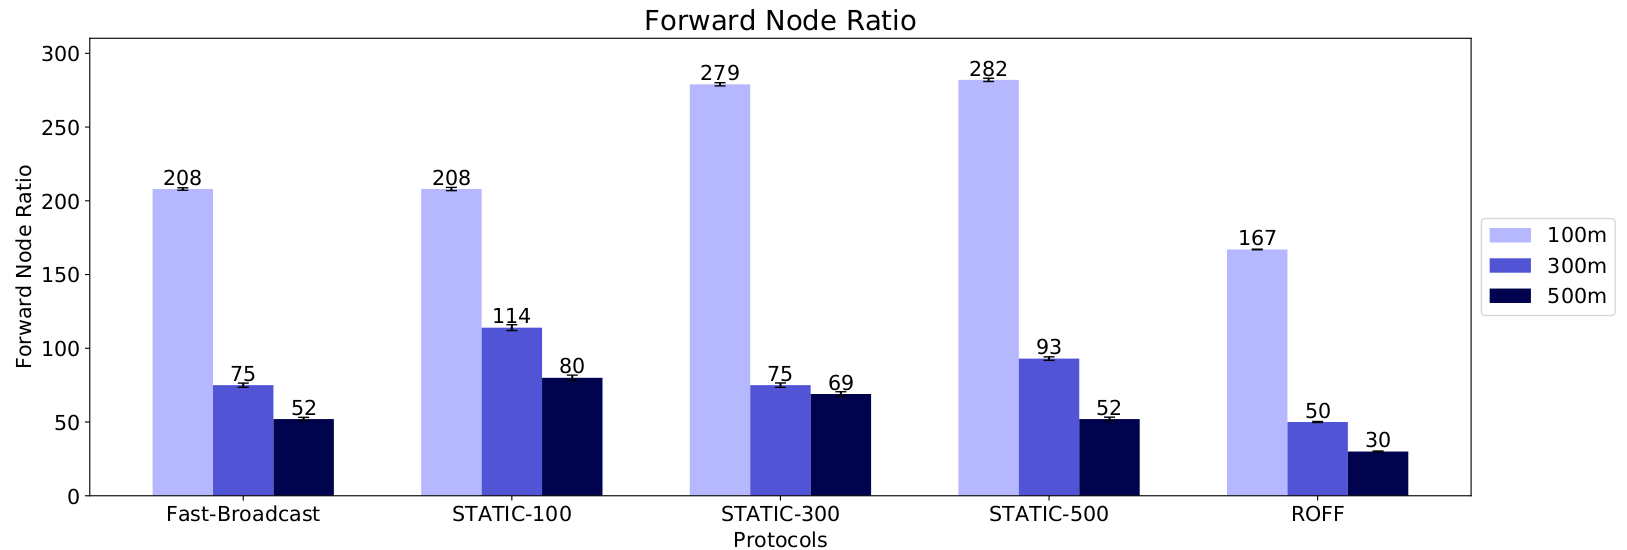
\includegraphics[width=1.1\textwidth]{immagini/platoon-15km/fnn}
			\caption{\textit{TDROC}, \textit{NOH}, \textit{NOS} and \textit{FNN} metrics for Platoon scenario}
			\label{fig:metric-platoon-15km-1}
		\end{figure}
	
		\newpage
	
		Since this scenario is one-dimensional, the circumference simply consists in vehicles distant $14.000  \pm 25$ meters from the source of Alert Message. Both metrics about delivery ratios (global and on circumference) are exactly 100\%, so the algorithms successfully propagate the \acrshort{ama} until the end of the platoon.
		
		
		Considering the Number Of Hops, ROFF's results are 11.76\%, 6.54\% and 9.08\% lower than Fast-Broadcast's results respectively for 100, 300 and 500 meters transmission range. ROFF's results are close to the optimal number of hops, respectively 140, 46.6 and 28 for the same transmission ranges as above. This means that the forwarder selection algorithms based on ESD Bitmap works better at choosing the farthest vehicle from the previous forwarder compared to the contention window approach for 1D scenarios. Considering STATIC variants of Fast-Broadcast, it is possible to observe that the STATIC-tx variant produces comparable results with Fast-Broadcast with \textit{tx} transmission range (e.g. STATIC-100 value is comparable to Fast-Broadcast with 100 meters transmission range), as expected. The STATIC protocol performs worse (hence the Number of Hops increases) whenever the transmission range is underestimated (e.g. STATIC-100 with 300 meters transmission range, compared to Fast-Broadcast with the same transmission range) or overestimated (e.g. STATIC-500 with 100 meters transmission range, compared to Fast-Broadcast with the same transmission range). This behaviour is expected, as reported in \cite{BAR2017}.
		
		
		Regarding the Number of Slots, ROFF performs much better than Fast-Broadcast. The metric's value is decreased respectively by 97.92\%, 92.27\% and 90.85\% using ROFF. The waiting time calculation, based on unique forwarding priority instead of distance, guarantees a much lower wait compared to Fast-Broadcast's contention window approach. As before, STATIC approaches produce results comparable with Fast-Broadcast when the transmission range estimation is correct. Instead, the Number of Slots greatly increases when the transmission range is underestimated and decreases when the transmission range is overestimated. In this last case, the decrease in \textit{NOS} comes with an increase in Number Of Hops reported in the previous paragraph, so an overestimation of transmission range is not desirable.
		
		
		Lastly, it is possible to see that ROFF achieves a better suppression of redundant transmissions, guaranteeing a decrease of 19.71\%, 33.33\% and 42.31\% respectively for each one of the transmission ranges considered.
		
		
	\section{Grid scenario}
		\label{sec:grid}
		After tests on the 1D Platoon scenario have been carried out, the next step consisted in testing the algorithms' performances in a two-dimensional Grid scenario, employing also the shadowing model introduced in \ref{sec:shadowing}. The Grid scenario consisted in a grid built by 17 north-south and 17 west-east roads, distant 300 meters from each other. Each road is 10 meters wide. Vehicles are placed only inside roads and are 25 meters distant from each other. The source of the Alert Message is in the middle of the grid, and the circumference has a radius of 2000 meters. For metrics calculation, vehicles are considered inside the circumference if they are $2000 \pm 25$ meters far from the source. Buildings are placed inside the blocks generated by road intersections, and are square shaped with an edge of 290 meters.
		
		
		Parameters for this scenario are included in Table \ref{tab:grid}.  
		
		\begin{table}[H]
			\def\arraystretch{1.1}
			\rowcolors{2}{D}{P}	
			\begin{tabularx}{\textwidth}{l | l  l}
				\rowcolor{I} {\large \textcolor{white}{Parameter}} & {\large \textcolor{white}{Value}} & {\large \textcolor{white}{}} \TBstrut  \\
				\toprule
				\endhead
				%			\midrule[1pt]
				\rowcolor{P} \multicolumn{3}{c}{Scenario configuration} \\
				\midrule[1pt]
				Road length 							& 4800	 				& m		\\
				Distance between roads					& 300					& m		\\
				Road width								& 10					& m		\\
				Number of roads (vertical)				& 17					&		\\
				Number of roads (horizontal)			& 17					&		\\
				Distance between vehicles 				& 25					& m		\\
				Circumference radius					& 2000					& m		\\
				Number of vehicles						& 6528					& 		\\
				Source of alert message position		& Center				&		\\
				Edge of buildings						& 290					& m		\\
				Number of buildings						& 255					& m		\\
				\midrule[1pt]
				\rowcolor{P} \multicolumn{3}{c}{Simulator configuration} \\
				\midrule[1pt]
				Shadowing model							& Obstacle Shadowing	&		\\
				Junction modeling						& No					&		\\
				\midrule[1pt]
				Number of simulations per configuration	& 1000					&		\\
				\bottomrule
			\end{tabularx}
			\caption{Grid scenario configuration}
			\label{tab:grid}
		\end{table}
	
		\begin{figure}[H]
			\centering
			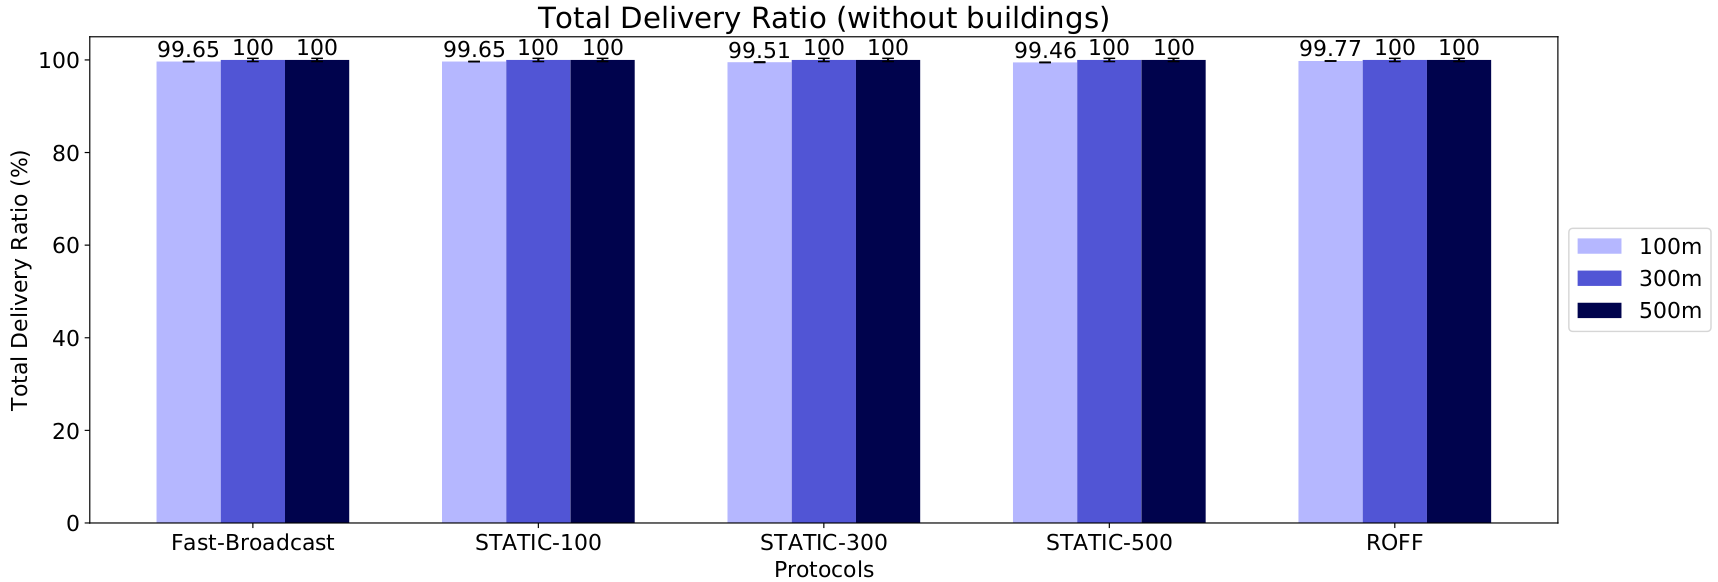
\includegraphics[width=1.0\textwidth]{immagini/grid-300/b0/tdr}
			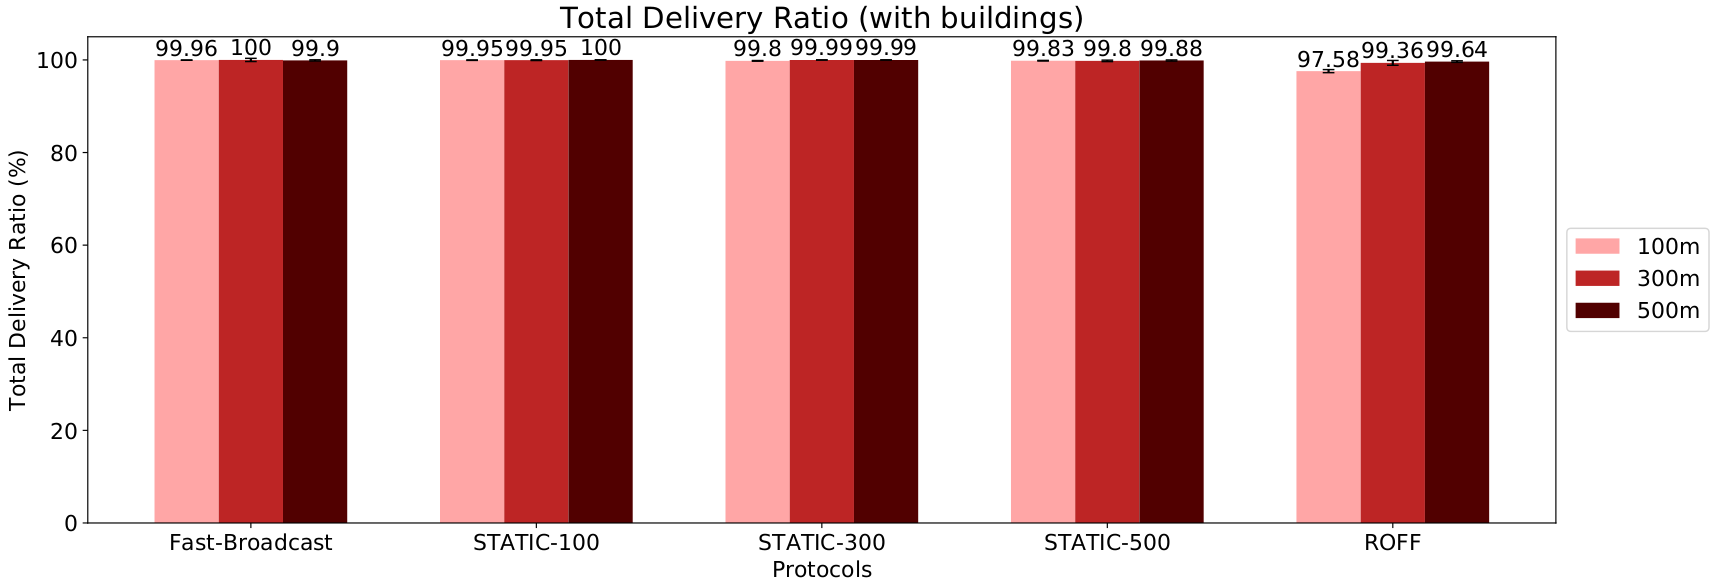
\includegraphics[width=1.0\textwidth]{immagini/grid-300/b1/tdr}
			\caption{\textit{TDR} without buildings (top) and with buildings (bottom) for Grid scenario}
			\label{fig:grid-tdr}
		\end{figure}
		
		\begin{figure}[H]
			\centering
			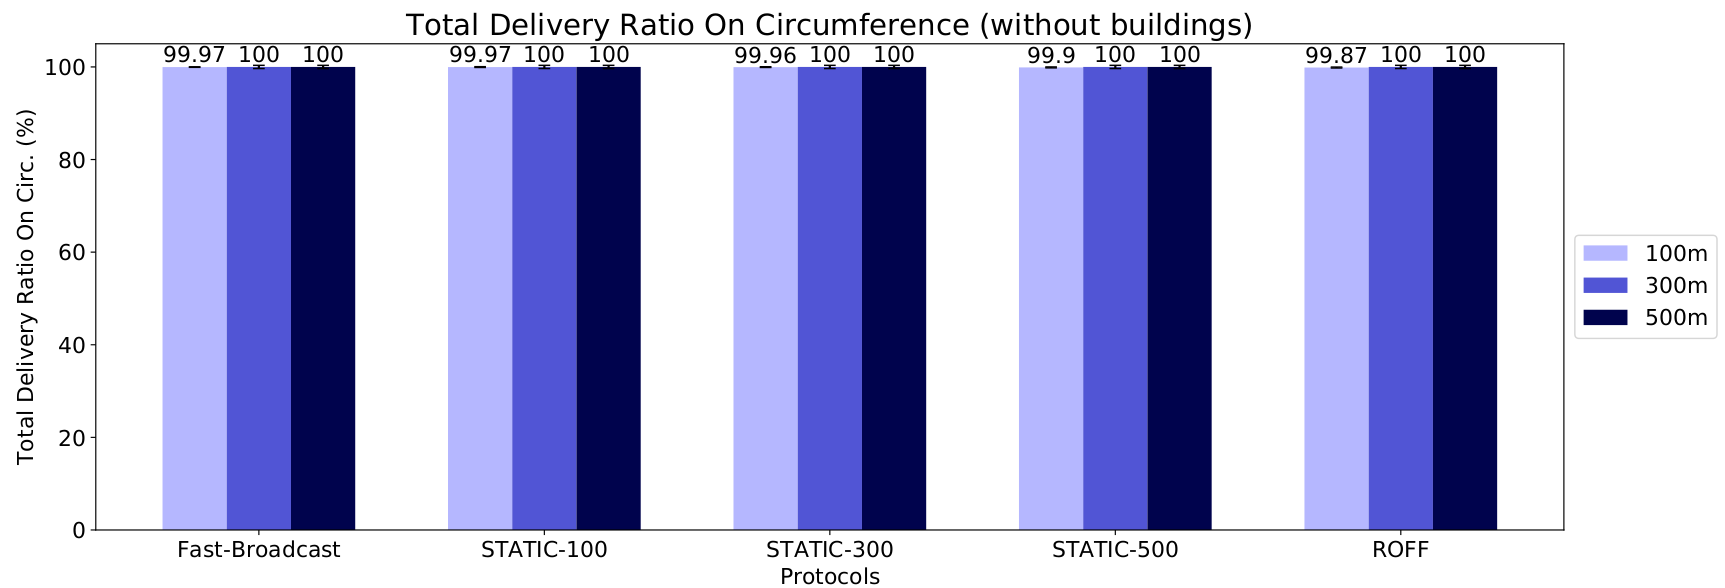
\includegraphics[width=1.0\textwidth]{immagini/grid-300/b0/tdroc}
			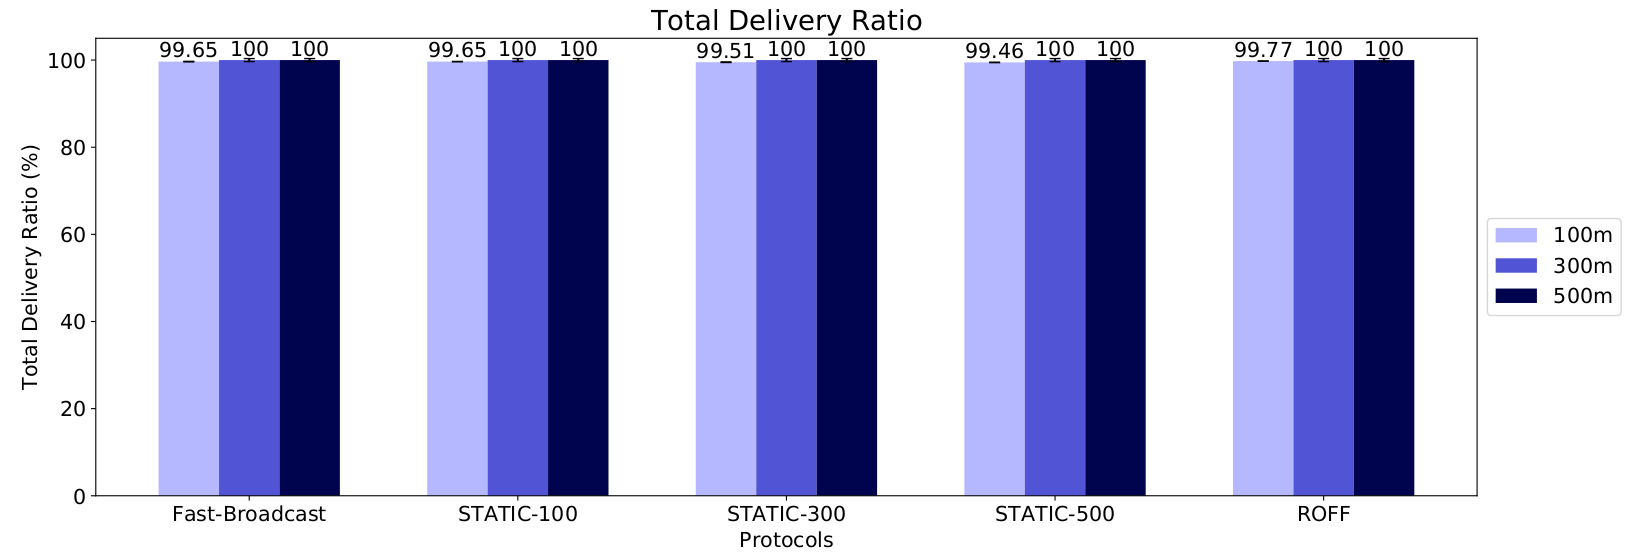
\includegraphics[width=1.0\textwidth]{immagini/grid-300/b1/tdroc}
			\caption{\textit{TDROC} without buildings (top) and with buildings (bottom) for Grid scenario}
			\label{fig:grid-tdroc}
		\end{figure}
	
		\begin{figure}[H]
			\centering
			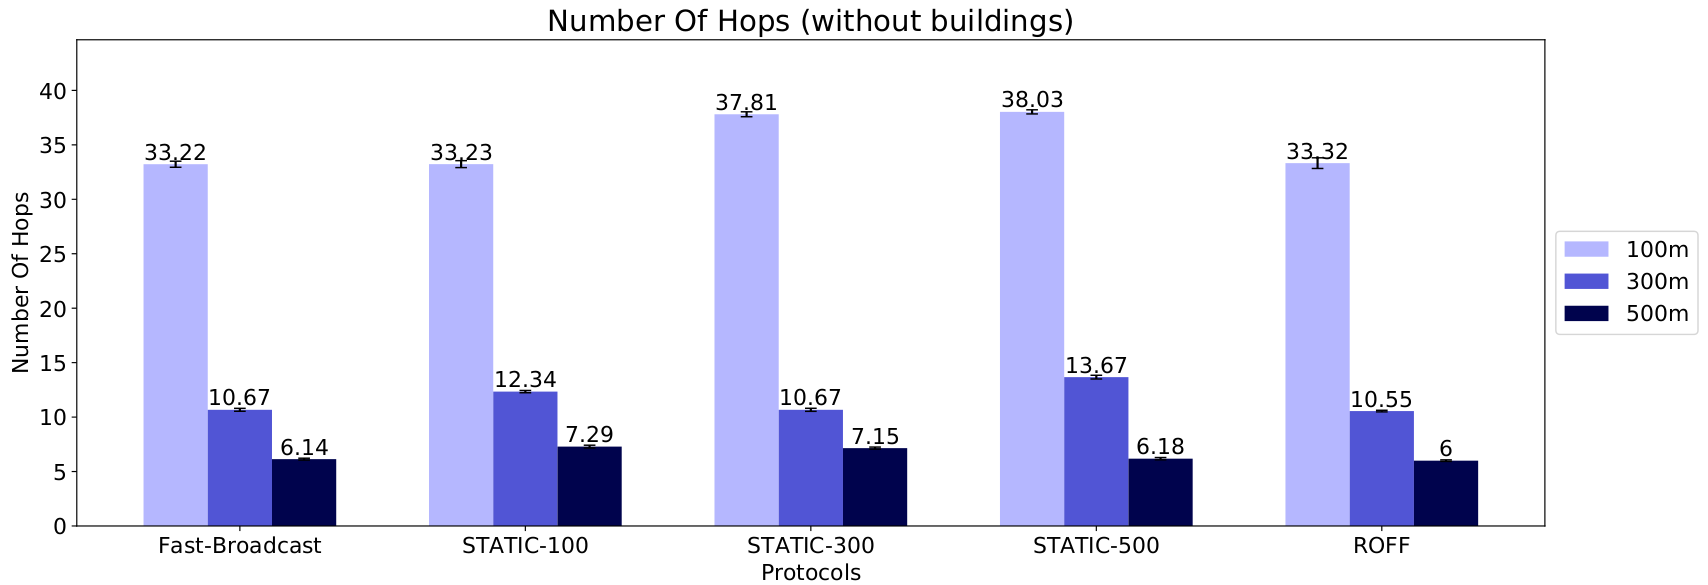
\includegraphics[width=1.0\textwidth]{immagini/grid-300/b0/noh}
			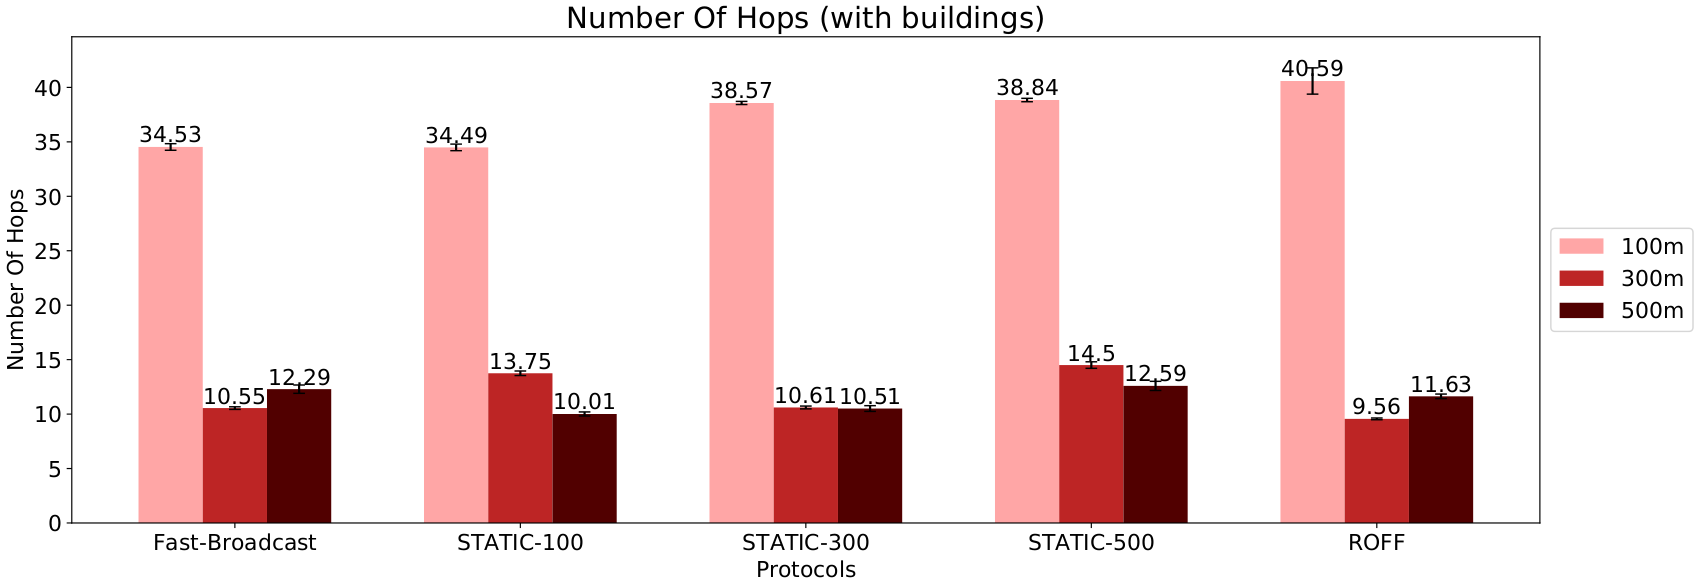
\includegraphics[width=1.0\textwidth]{immagini/grid-300/b1/noh}
			\caption{\textit{NOH} without buildings (top) and with buildings (bottom) for Grid scenario}
			\label{fig:grid-noh}
		\end{figure}
	
		\begin{figure}[H]
			\centering
			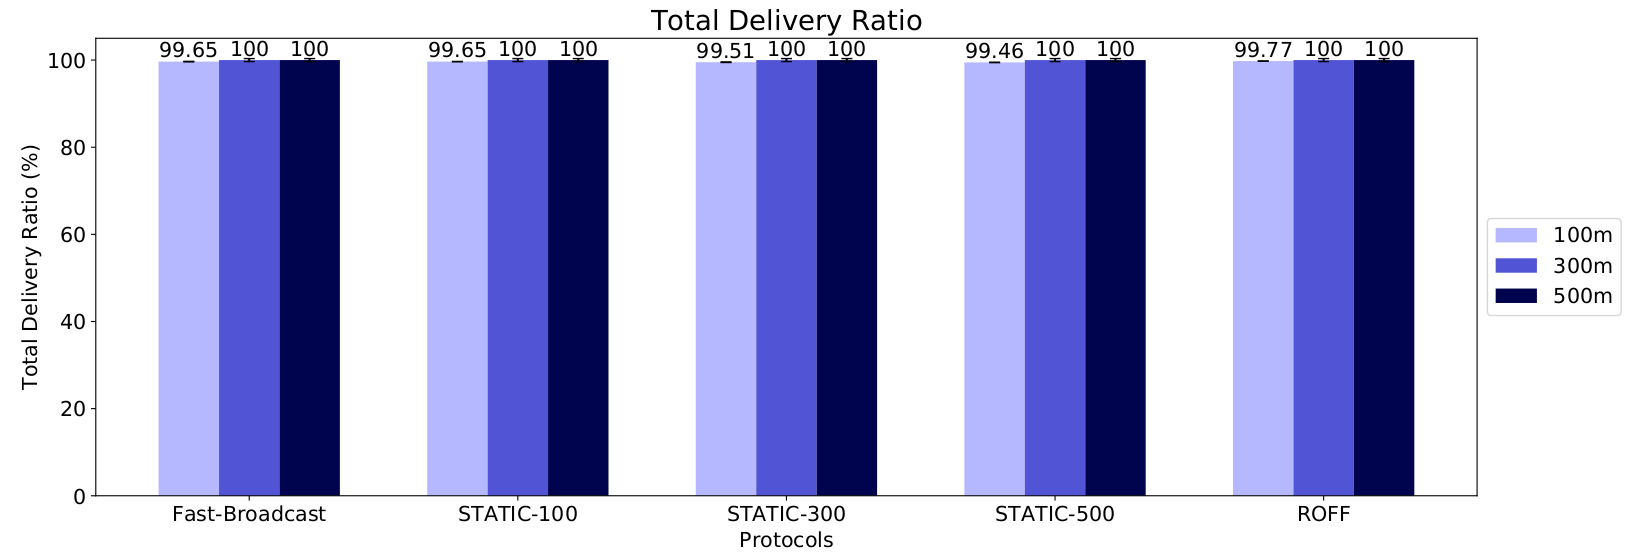
\includegraphics[width=1.0\textwidth]{immagini/grid-300/b0/nos}
			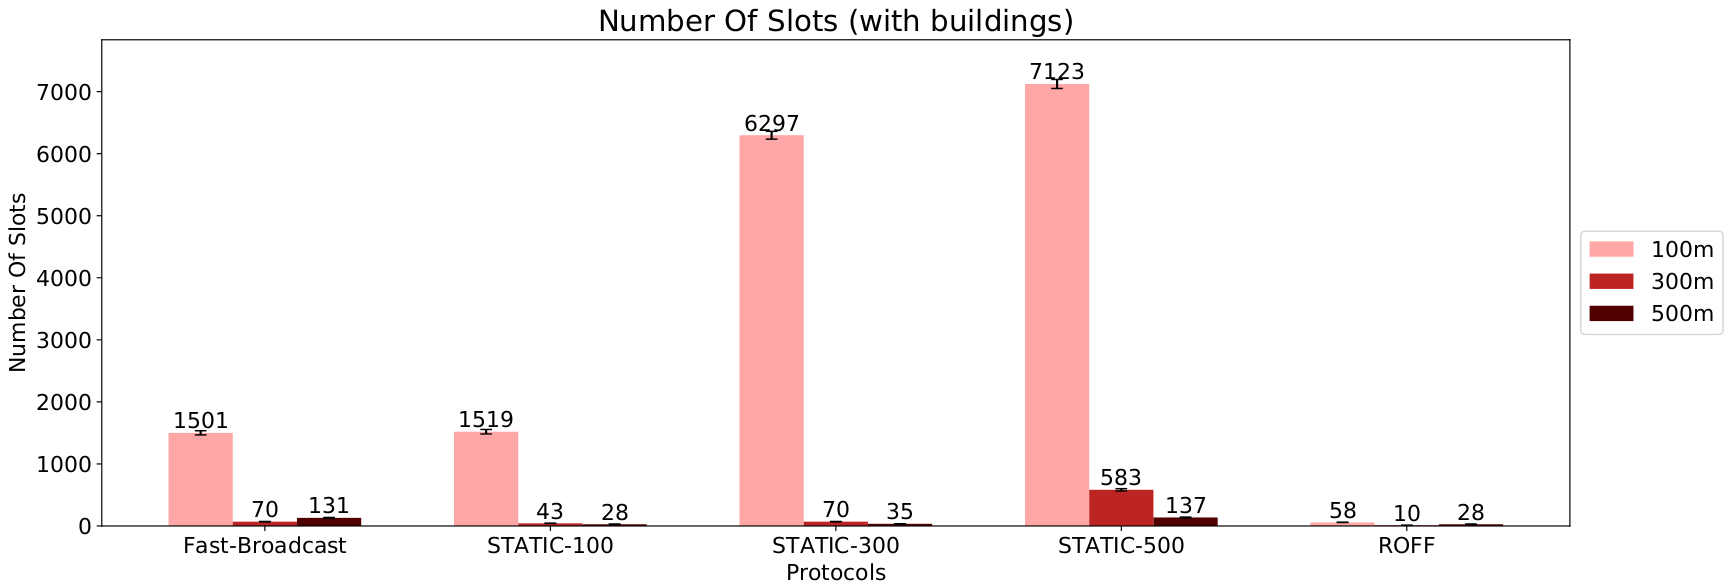
\includegraphics[width=1.0\textwidth]{immagini/grid-300/b1/nos}
			\caption{\textit{NOS} without buildings (top) and with buildings (bottom) for Grid scenario}
			\label{fig:grid-nos}
		\end{figure}
	
		\begin{figure}[H]
			\centering
			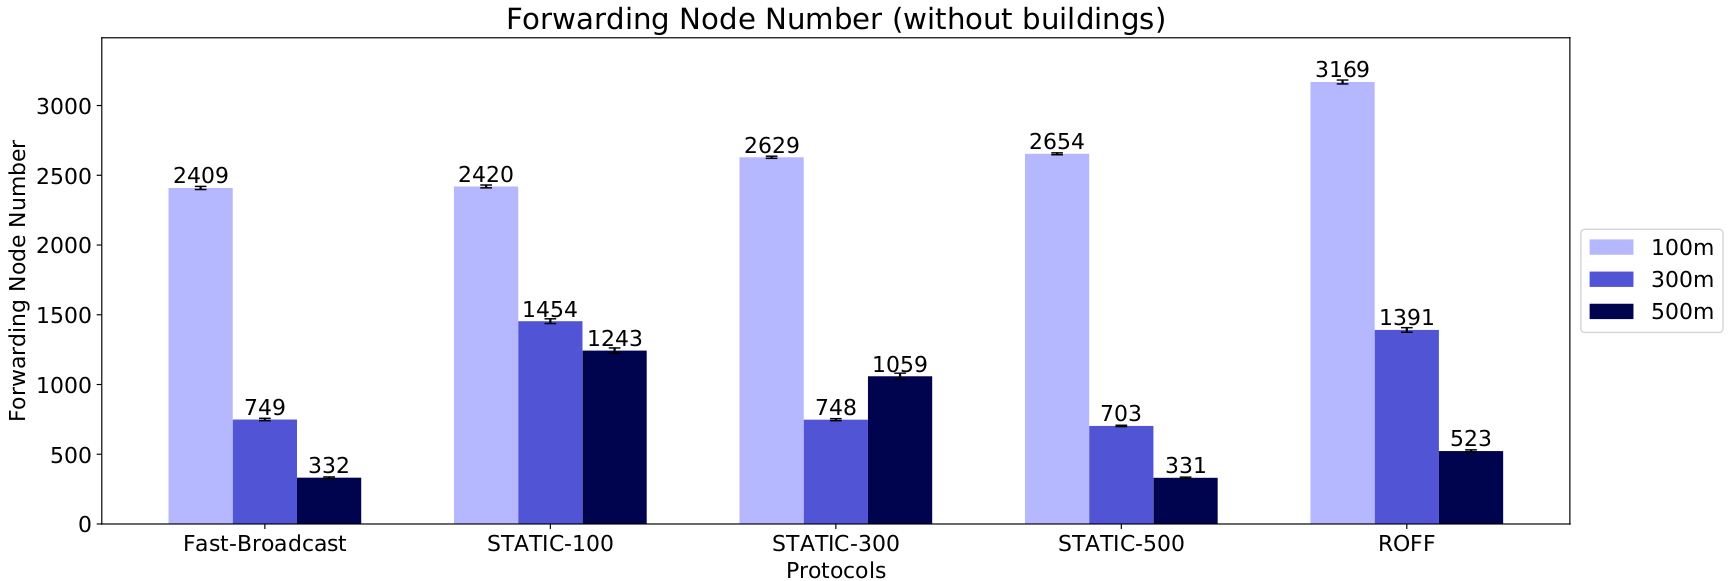
\includegraphics[width=1.0\textwidth]{immagini/grid-300/b0/fnn}
			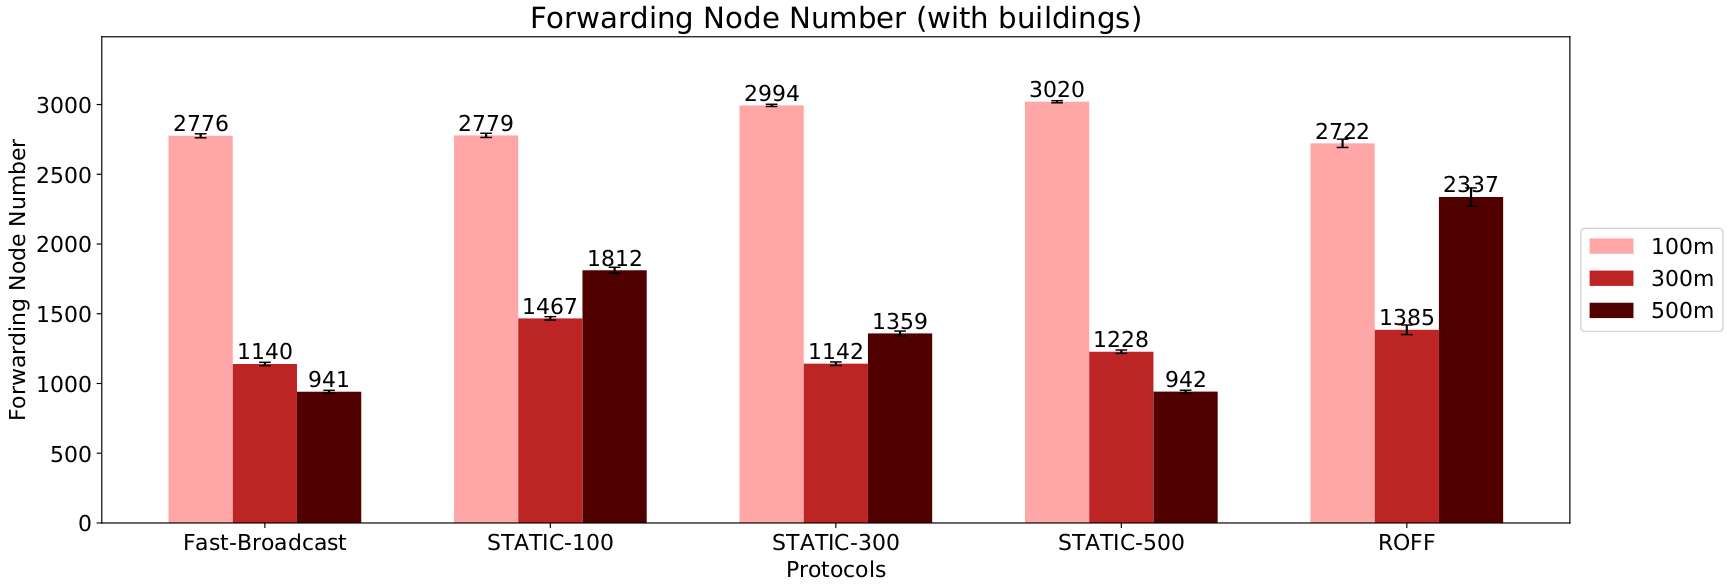
\includegraphics[width=1.0\textwidth]{immagini/grid-300/b1/fnn}
			\caption{\textit{FNN} without buildings (top) and with buildings (bottom) for Grid scenario}
			\label{fig:grid-fnn}
		\end{figure}
		
		\newpage
		
		All the algorithms perform well as far as delivery ratios are concerned (Figure \ref{fig:grid-tdr} and \ref{fig:grid-tdroc}), for both configurations with and without buildings. This means that the shadowing caused by the Obstacle Model does not create no-reach zones, and the signal manages to find its way to almost all of the vehicles. The regular pattern by which vehicles are placed may help with that: further testing where this hypothesis is removed will be presented in the next sections. Even though delivery ratios are unchanged, the effect of the Obstacle model can be observed qualitatively comparing Figure \ref{fig:fb-b0-grid-transmission} and \ref{fig:fb-b1-grid-transmission} for Fast-Broadcast, and Figure \ref{fig:roff-b0-grid-transmission} and \ref{fig:roff-b1-grid-transmission} for ROFF. The effects of obstacles on propagation cause the signal to travel only through roads segments where line of sight is possible. Instead, without obstacles the signal can be propagated freely in all directions.
		
		
		Moreover, Fast-Broadcast and ROFF can be compared with each other by looking at Figure \ref{fig:fb-b0-grid-transmission} and \ref{fig:roff-b0-grid-transmission} for the scenario without buildings, and Figure \ref{fig:fb-b1-grid-transmission} and \ref{fig:roff-b1-grid-transmission} for the scenario with buildings. In both cases, ROFF designates the farthest PFC as the next forwarder much more reliably than Fast-Broadcast thanks to the Neighbor Table mechanism. Instead, Fast-Broadcast relies on a random choice of waiting time, so the next designated forwarder is sometimes not one of the farthest vehicles from the previous forwarder. Based on this observation, we can expect a much lower NOH value for ROFF. Quantitative analysis of this and other metrics will be reported in the next paragraphs of this section.
		
		\begin{figure}[H]
			\centering
			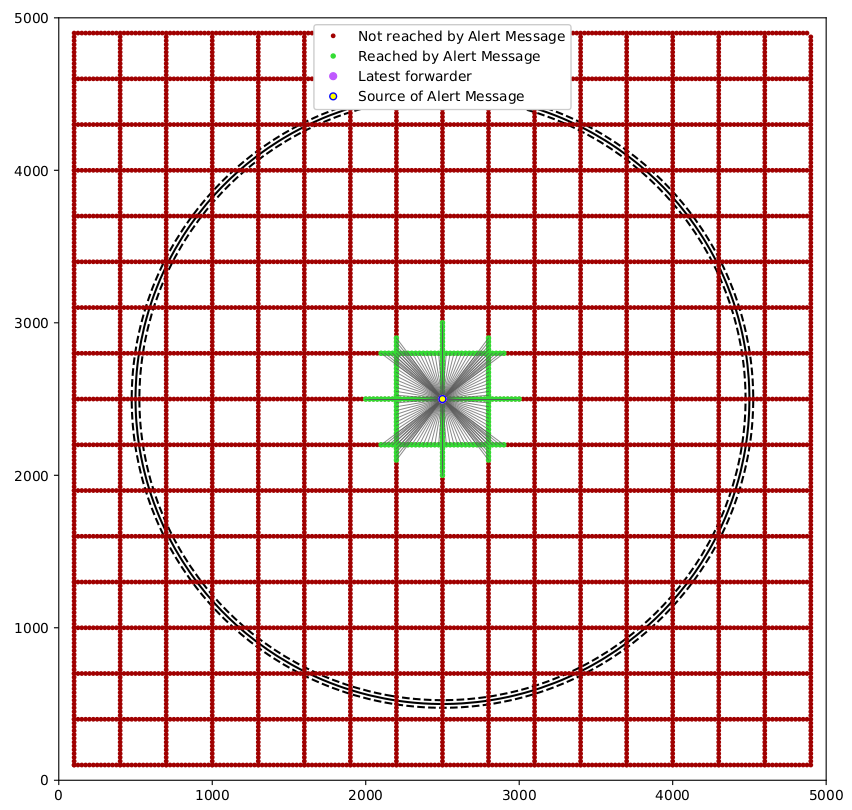
\includegraphics[width=0.8\textwidth]{immagini/grid-300/b0/fb-1hop}
			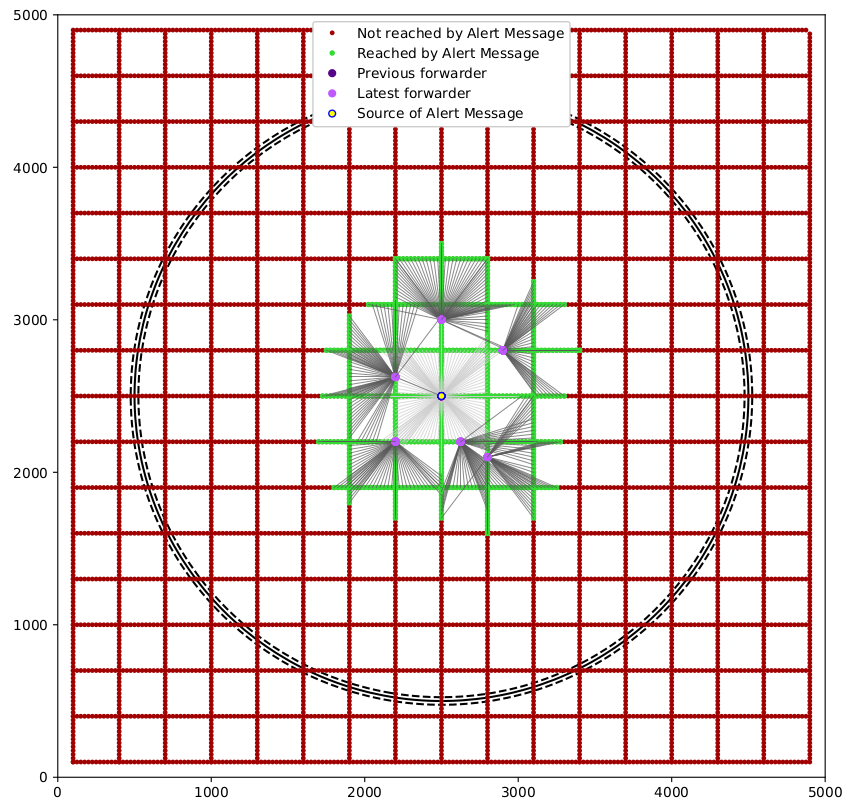
\includegraphics[width=0.8\textwidth]{immagini/grid-300/b0/fb-2hop}
			\caption{Fast-Broadcast after 1 hop (top) and 2 hops (bottom) in Grid scenario with 500 meters transmission range and without the Obstacle model}
			\label{fig:fb-b0-grid-transmission} 
		\end{figure}
		
		\begin{figure}[H]
			\centering
			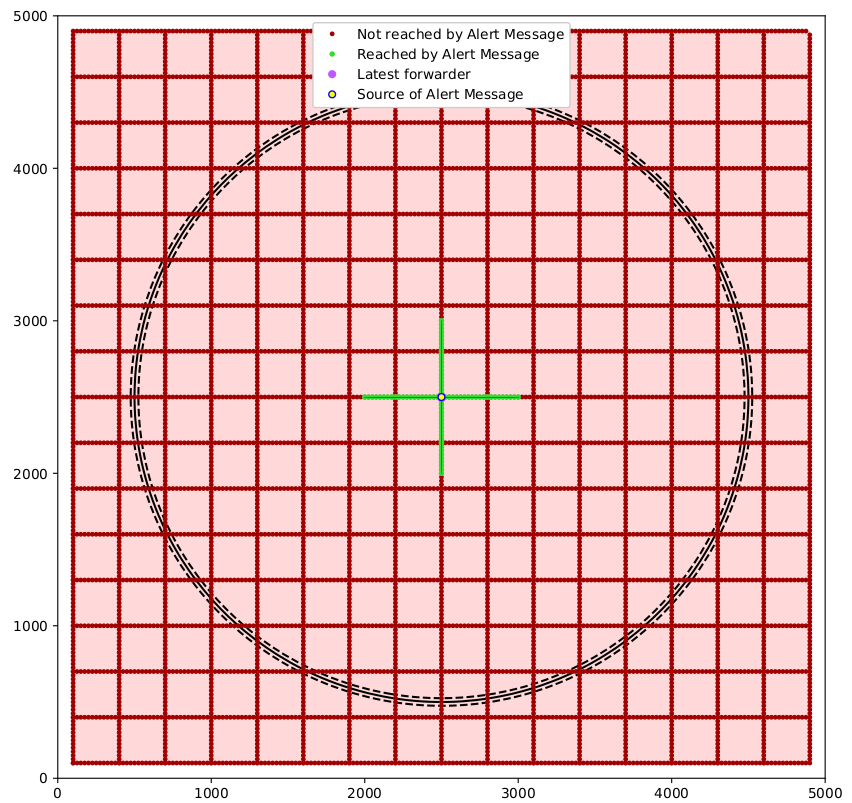
\includegraphics[width=0.8\textwidth]{immagini/grid-300/b1/fb-1hop}
			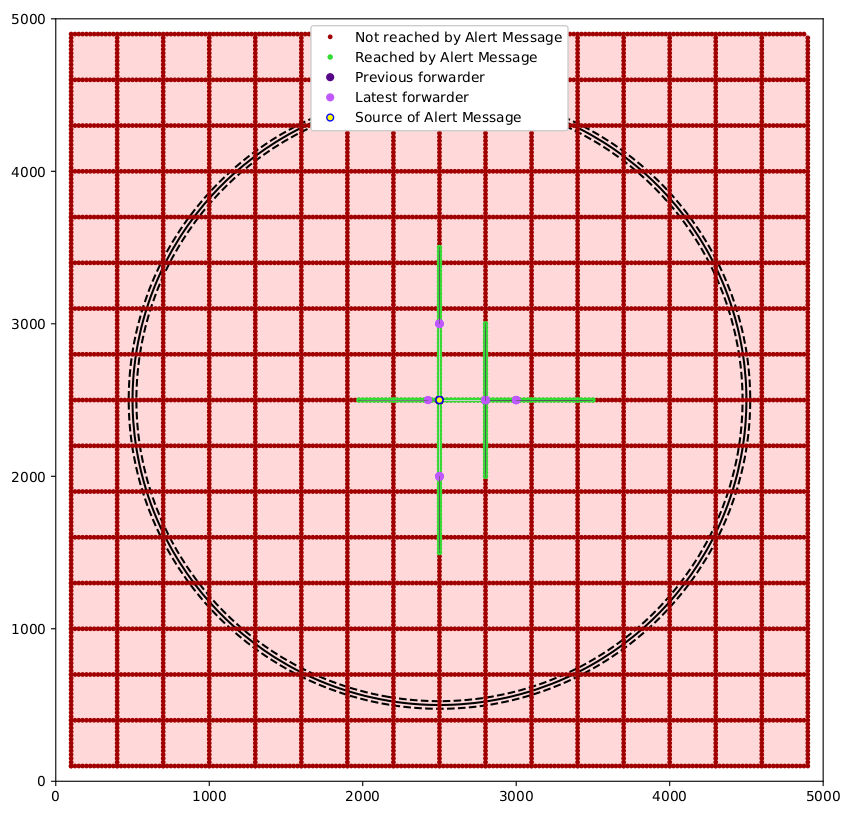
\includegraphics[width=0.8\textwidth]{immagini/grid-300/b1/fb-2hop}
			\caption{Fast-Broadcast after 1 hop (top) and 2 hops (bottom) in Grid scenario with 500 meters transmission range and with the Obstacle model}
			\label{fig:fb-b1-grid-transmission} 
		\end{figure}
	
		\begin{figure}[H]
			\centering
			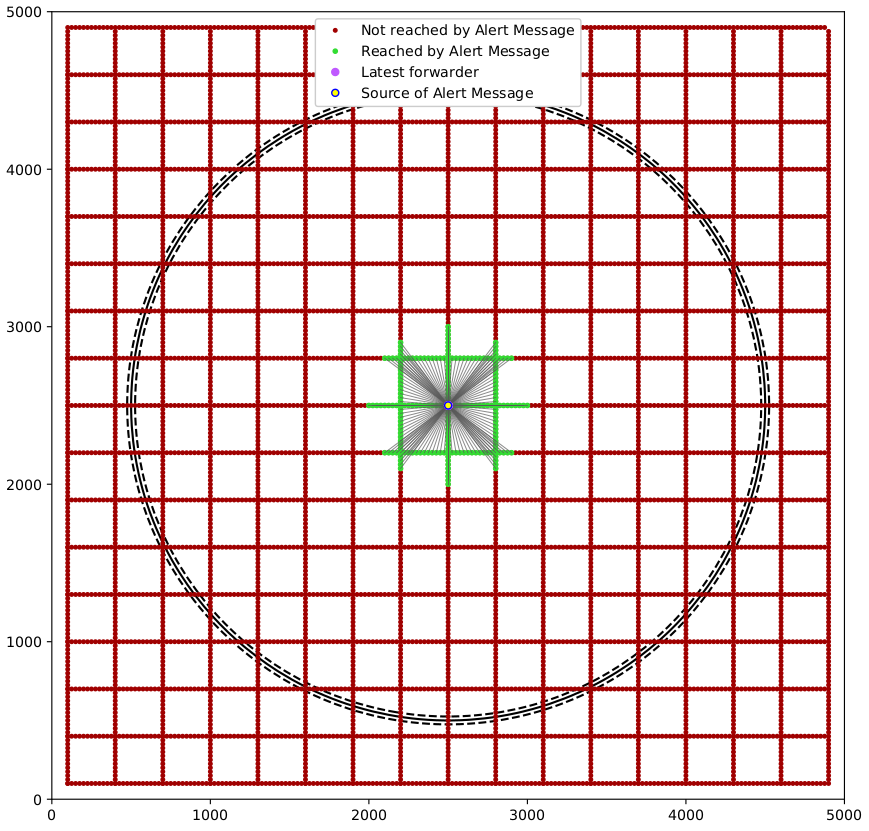
\includegraphics[width=0.8\textwidth]{immagini/grid-300/b0/roff-1hop}
			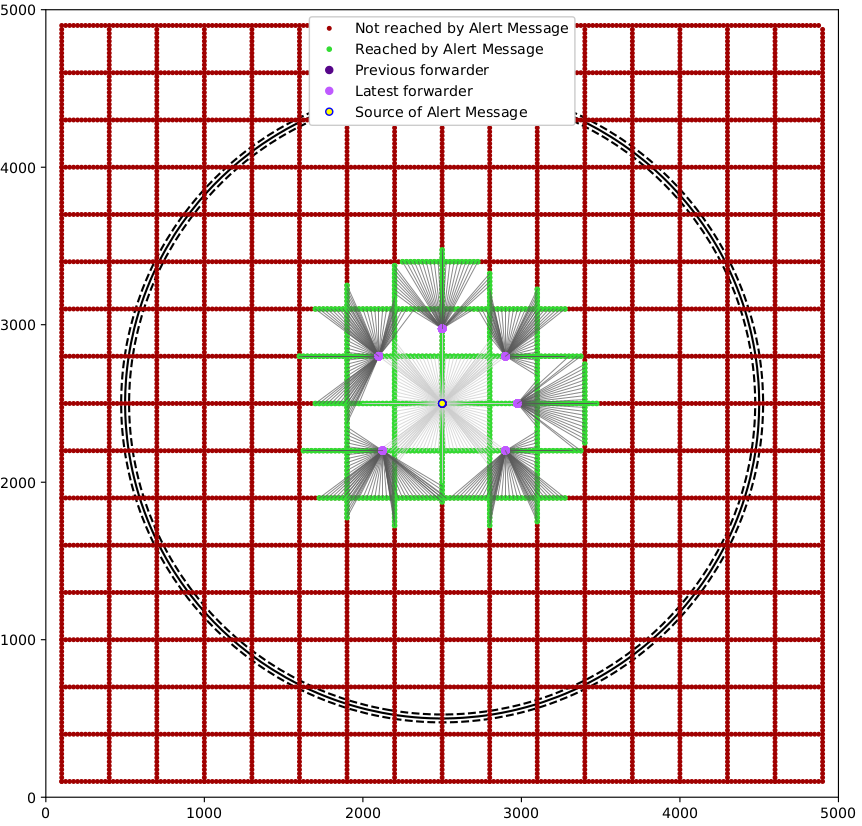
\includegraphics[width=0.8\textwidth]{immagini/grid-300/b0/roff-2hop}
			\caption{ROFF after 1 hop (top) and 2 hops (bottom) in Grid scenario with 500 meters transmission range and without the Obstacle model}
			\label{fig:roff-b0-grid-transmission}
		\end{figure}
	
		\begin{figure}[H]
			\centering
			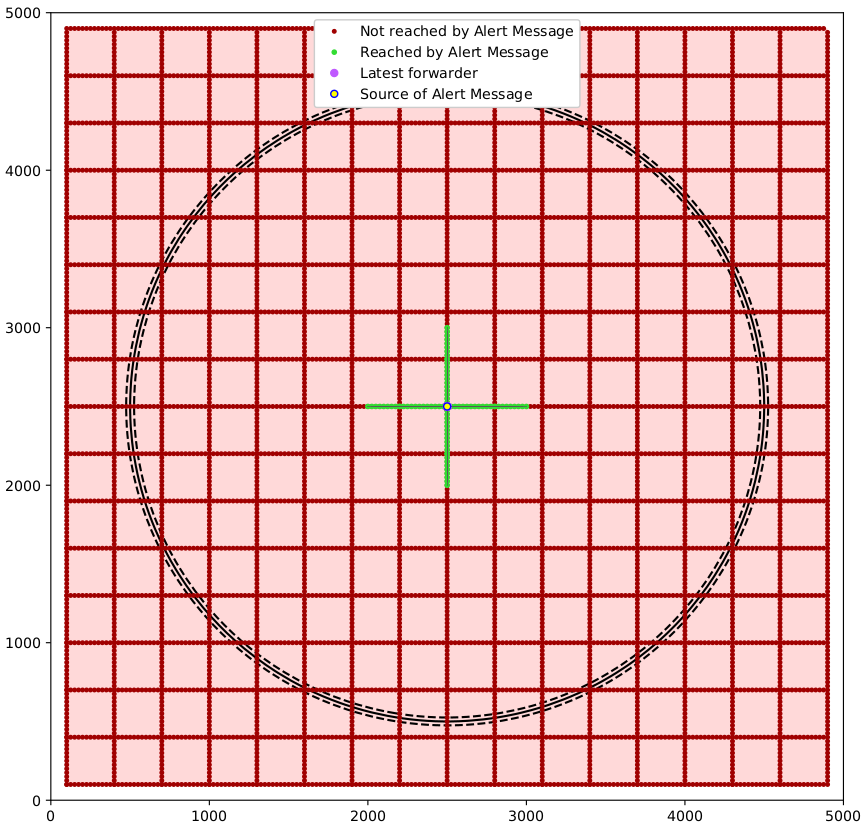
\includegraphics[width=0.8\textwidth]{immagini/grid-300/b1/roff-1hop}
			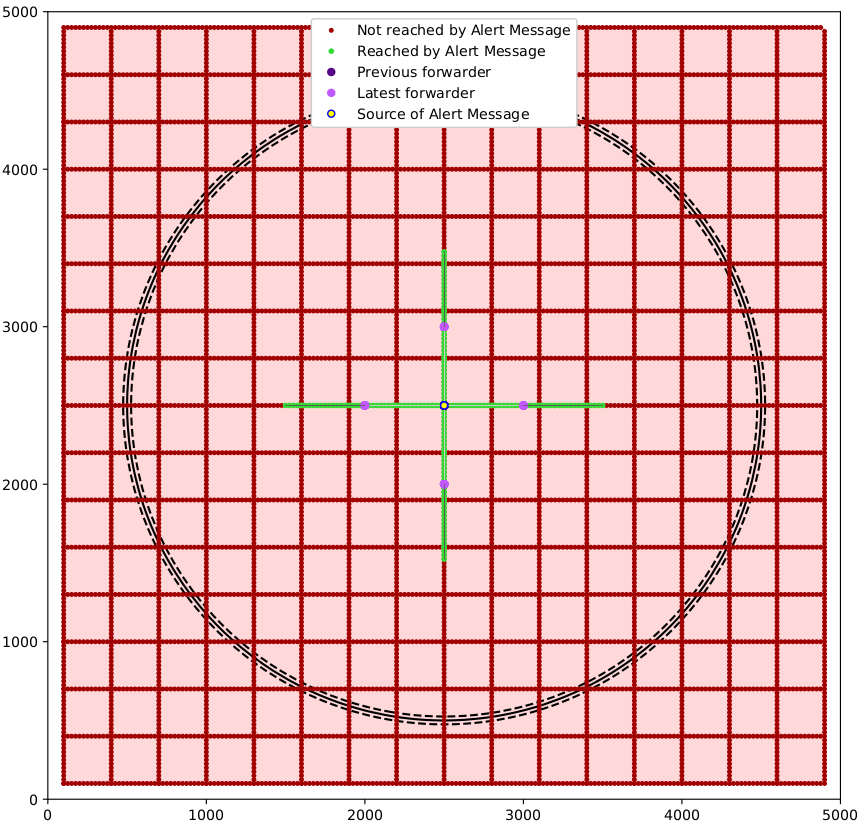
\includegraphics[width=0.8\textwidth]{immagini/grid-300/b1/roff-2hop}
			\caption{ROFF after 1 hop (top) and 2 hops (bottom) in Grid scenario with 500 meters transmission range and with the Obstacle model}
			\label{fig:roff-b1-grid-transmission}
		\end{figure}
		
		If we focus on the Number Of Hops (Figure \ref{fig:grid-noh}), we notice that the introduction of buildings causes the number of hops to increases for transmission ranges of 100 and 500 meters, while decreases for 300 meters tranmission range. This is probably due to the fact that the distance between roads is also 300 meters and the starting vehicle is inside a junction. This means that the effect of buildings causes the signal to travel along roads, hopping from junction to junction, and reaching the circumference much faster. Another unusual observervation consists in ROFF with 100 meters transmission range, where the value increases by a lot. This case needs further examination in order to be explained. Apart from this case, ROFF achieves better results than Fast-Broadcast, with results 9\% and 3.47\% better for 300 and 500 meters transmission range respectively. 
		
		
		The analysis of the Number Of Slots (Figure \ref{fig:grid-nos}) shows similar results: the shadowing model causes the metric's value to rise in all configurations except for ROFF with 300 meters transmission range. ROFF continues to outperform Fast-Broadcast with results similar to those observed in the Platoon scenario. 
		
		
		Considering the Forwarding Node Number (Figure \ref{fig:grid-fnn}), the situation is much different than the previous scenario. It is possible to see in both graphs that ROFF's values are higher than Fast-Broadcast's across all configurations. Despite the almost-perfect suppression of redundant transmission works in a 1D scenario, as observed in the previous section, the mechanism does not seem to have much of an effect in a 2D scenario, regardless of the presence of buildings. A possible explanation of this phenomenon might be the one reported in Figure \ref{fig:2d-roff}, which indicates a possible Alert Message propagation process. Suppose that S is the previous forwarder: the other nodes on the circumference (distant txRange from S) are the elected FFCs which win the contention and relay the message. Due to how ROFF works, those nodes send the message at exactly the same time, hence if we focus on A and B we have a guaranteed collision area (the red area in Figure \ref{fig:2d-roff}). The nodes inside that collision area receive the forwarding from A and B at the same time and a collision occurs. As a consequence, they are not aware that the message has already been forwarded and some of them will fire their transmission. This process is repeated for every forward (and also for other FFCs other than A and B in the example) and so this could cause the increase in the FNN value. In other words, ROFF is guaranteed to cause the collision area shown in the example due to the exact waiting time calculation for nodes at the same distance from S. Fast-Broadcast is less affected by this problem since the waiting time calculation is not deterministic (the waiting time is chosen randomly from the interval [1...CW] where CW is calculated using Formula \ref{eq:contention-window}).
	
		\begin{figure}[H]
			\centering
			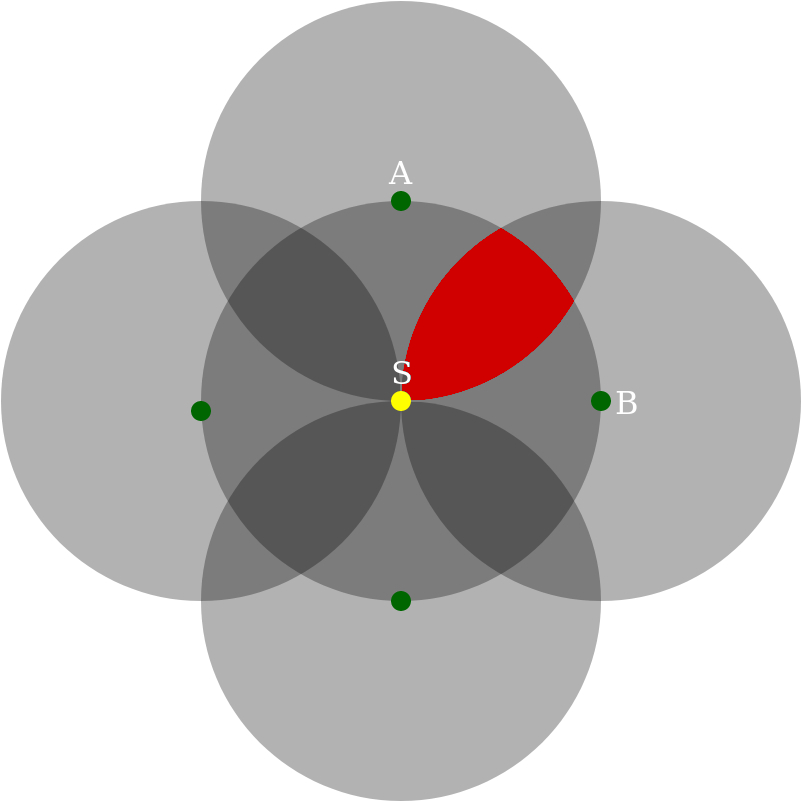
\includegraphics[width=0.5\textwidth]{immagini/2d-roff}
			\caption{Collision area in 2D scenarios for ROFF}
			\label{fig:2d-roff}
		\end{figure}

	\section{Los Angeles urban scenario}
		\label{sec:la-scenario}
		The next step consisted in expanding the 2D scenario with realistic urban data taken from OpenStreetMap and processed by SUMO as explained in Section \ref{sec:sumo}. In addition to the shadowing model, in this scenario (and also in the urban scenario regarding Padua, which will be presented in the next section), a \textit{smart junction} variant of the algorithms has been introduced in order to try to increase delivery ratios. 
		
		Figure \ref{fig:la-scenario} depicts the scenario with vehicles (green dots), buildings (pink polygons) and junctions (yellow polygons).
		
		
		All configurations are reported in Figure \ref{fig:la-overview}. In order to facilitate the understanding of the various configurations, the following graphs will utilize shades of color similar to those reported in Figure \ref{fig:la-overview} (e.g. graphs with shades of blue will represent a scenario without buildings and without junctions, while shades of orange will represent a scenario with buildings and with junctions). Parameters for this scenario are included in Table \ref{tab:la-25}.  
		
		\begin{figure}[H]
			\centering
			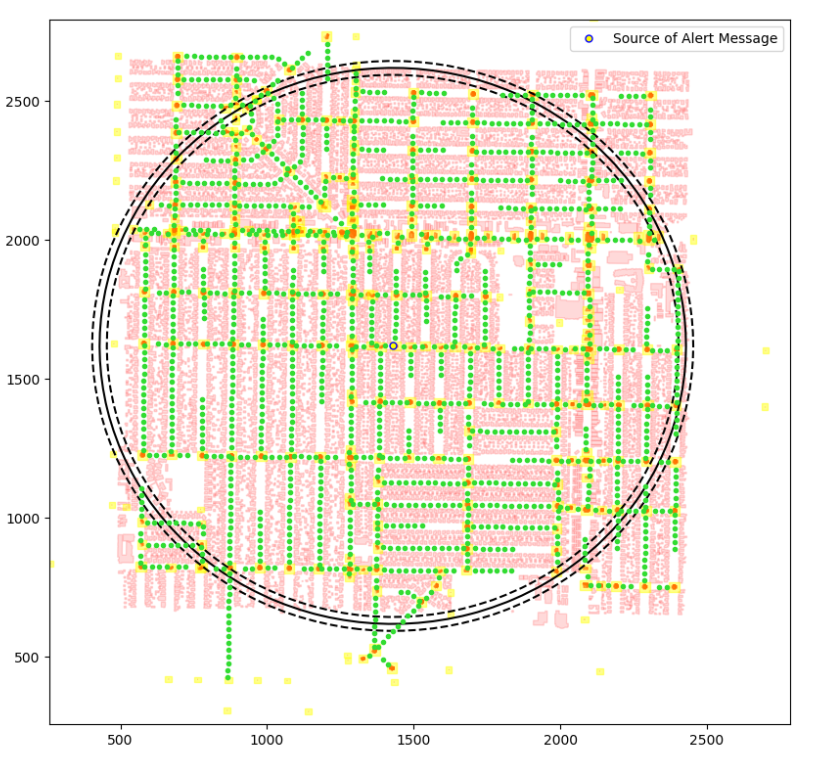
\includegraphics[width=0.90\textwidth]{immagini/la-25/la-scenario}
			\caption{Los Angeles urban scenario depiction}
			\label{fig:la-scenario}
		\end{figure}
		
		\begin{figure}[H]
			\centering
			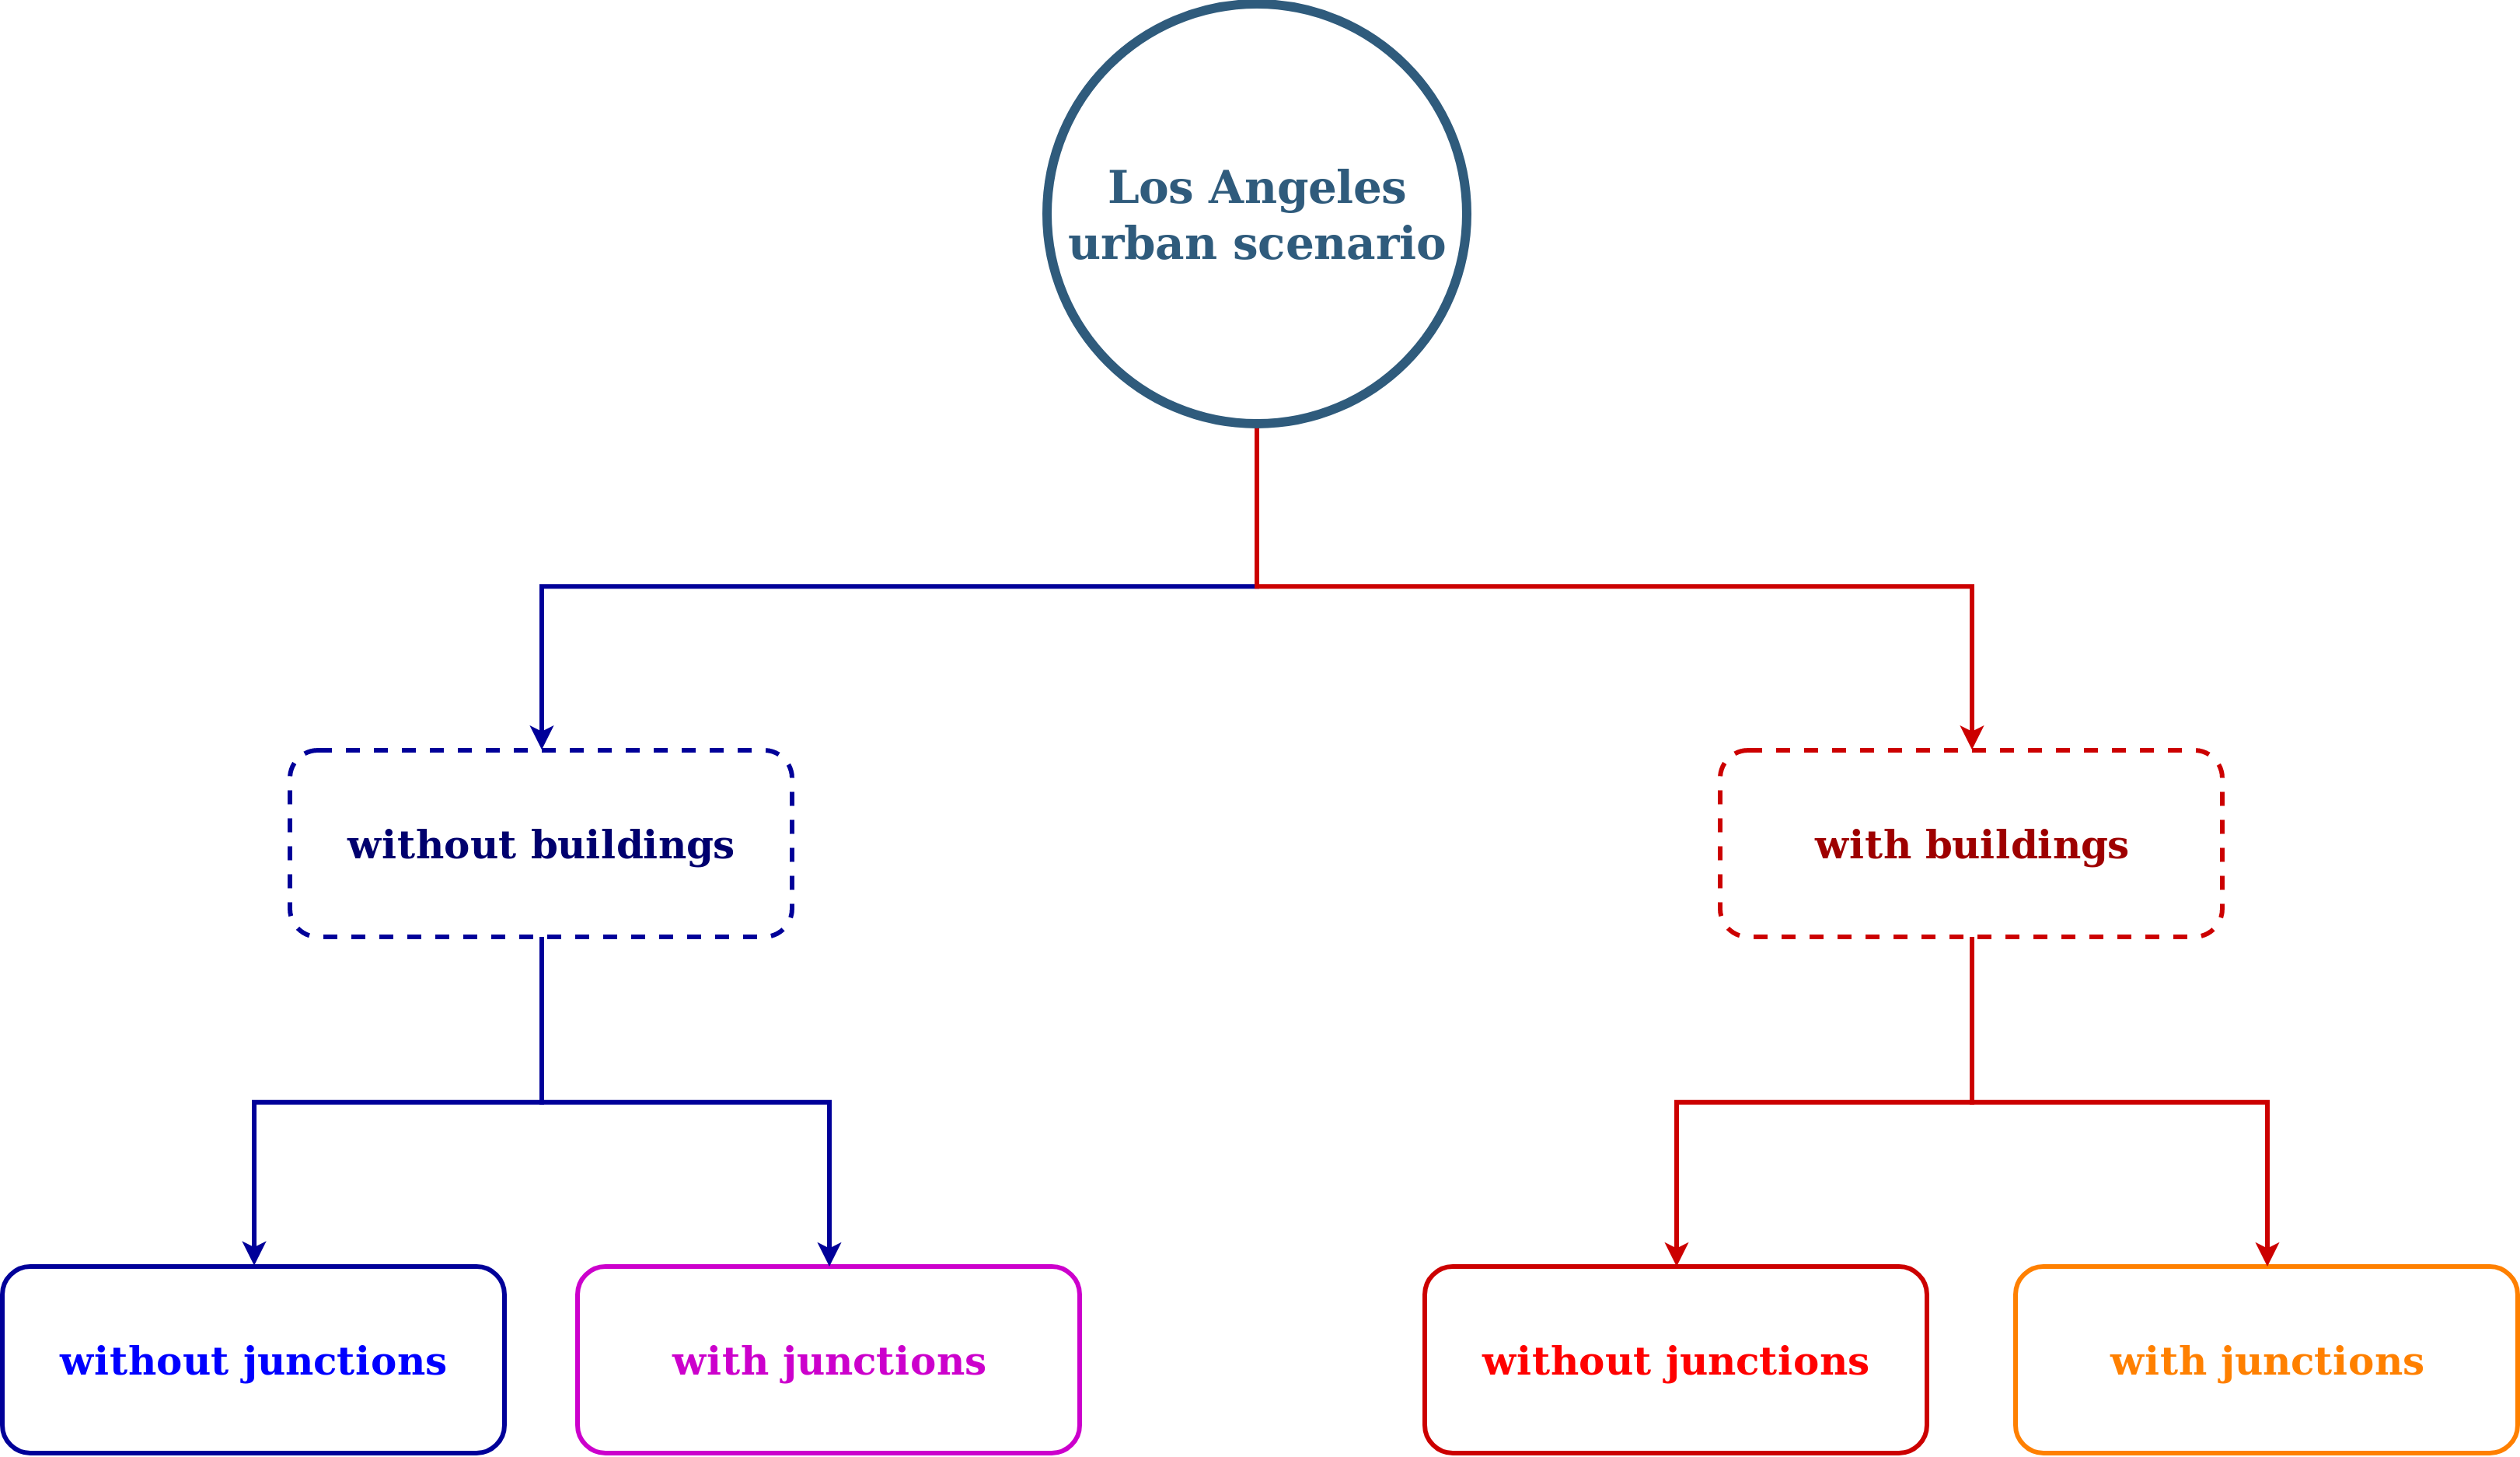
\includegraphics[width=1.0\textwidth]{immagini/la-25/overview}
			\caption{Los Angeles urban scenario test overview}
			\label{fig:la-overview}
		\end{figure}
	
		\begin{table}[H]
			\def\arraystretch{1.1}
			\rowcolors{2}{D}{P}	
			\begin{tabularx}{\textwidth}{l | l  l}
				\rowcolor{I} {\large \textcolor{white}{Parameter}} & {\large \textcolor{white}{Value}} & {\large \textcolor{white}{}} \TBstrut  \\
				\toprule
				\endhead
				%			\midrule[1pt]
				\rowcolor{P} \multicolumn{3}{c}{Scenario configuration} \\
				\midrule[1pt]
				Latitude N								& 33.9654				& \textdegree		\\
				Latitude S								& 33.9478				& \textdegree		\\
				Longitude W								& -118.3260				& \textdegree		\\
				Longitude E								& -118.3055				& \textdegree		\\
				Road length 							& 1200	 				& m		\\
				Distance between vehicles 				& 25					& m		\\
				Circumference radius					& 1000					& m		\\
				Number of vehicles						& 1465					& 		\\
				Source of alert message position		& Center				&		\\
				Number of buildings						& 8241					&		\\
				Number of junctions						& 1288					&		\\	
				\midrule[1pt]
				\rowcolor{P} \multicolumn{3}{c}{Simulator configuration} \\
				\midrule[1pt]
				Shadowing model							& Obstacle Shadowing 	&		\\
				Junction modeling						& Yes					&		\\
				\midrule[1pt]
				Number of simulations per configuration	& 4500					&		\\
				\bottomrule
			\end{tabularx}
			\caption{Los Angeles urban scenario configuration}
			\label{tab:la-25}
		\end{table}
	
		\begin{figure}[H]
			\centering
			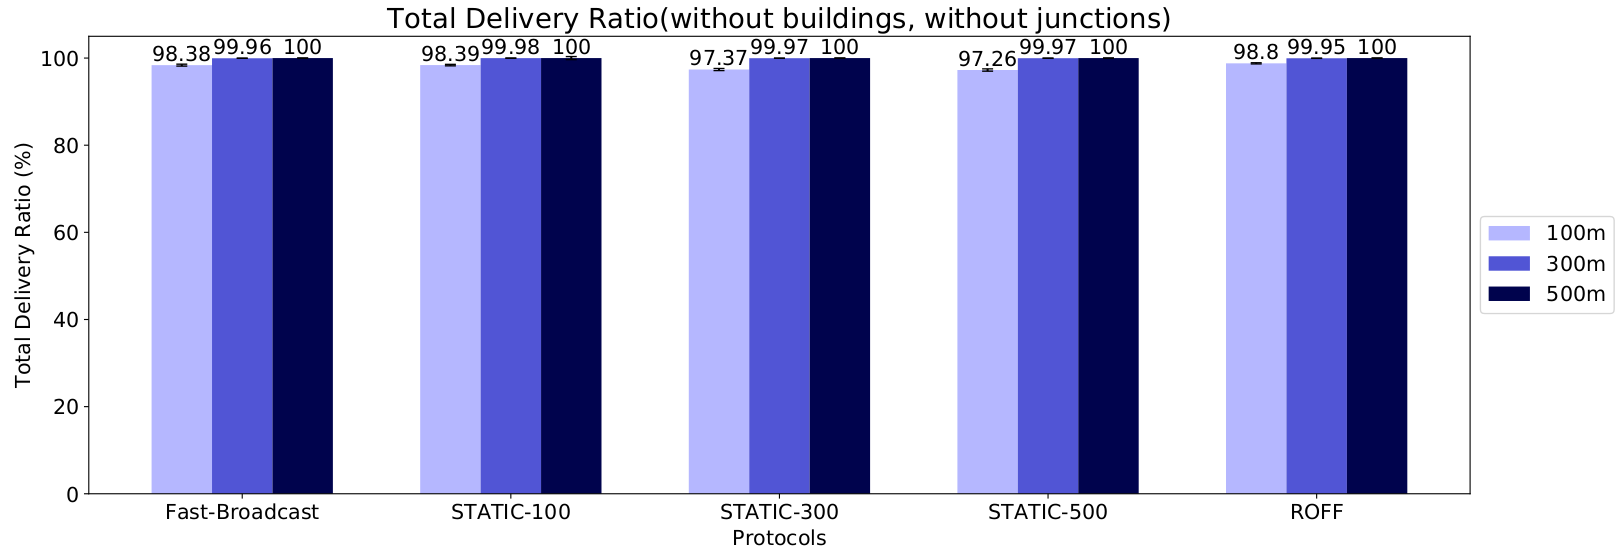
\includegraphics[width=1.0\textwidth]{immagini/la-25/b0/j0/tdr}
			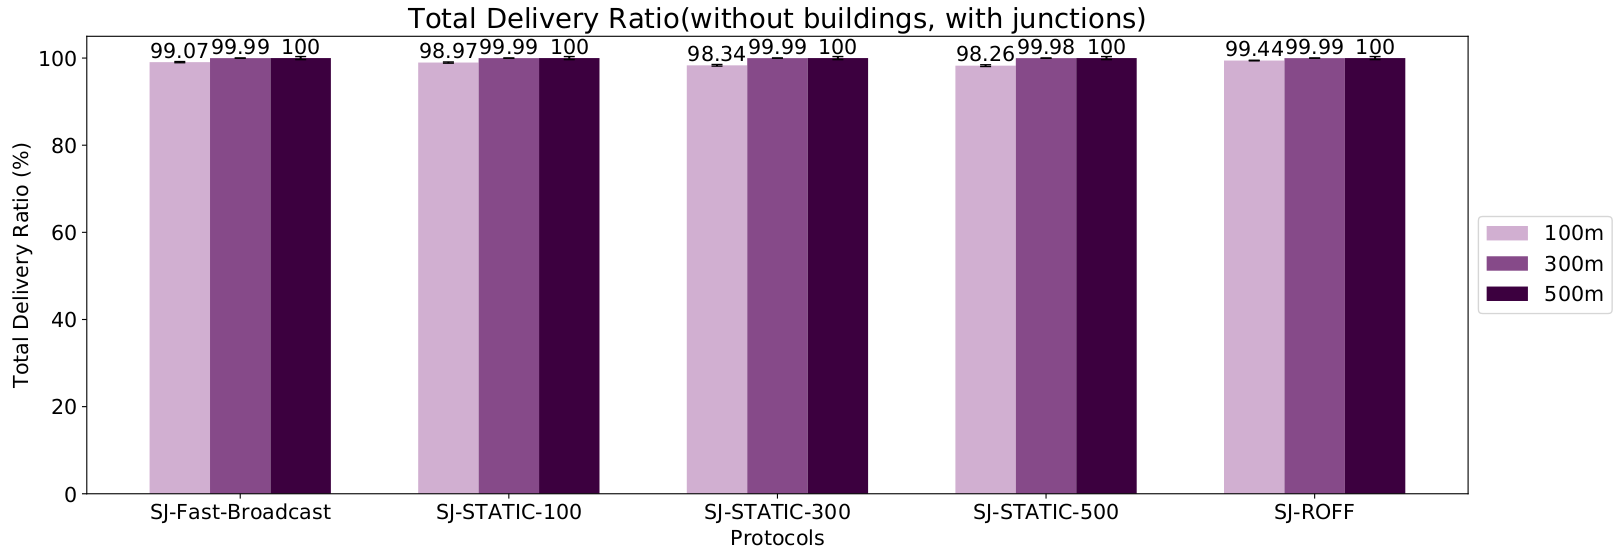
\includegraphics[width=1.0\textwidth]{immagini/la-25/b0/j1/tdr}
			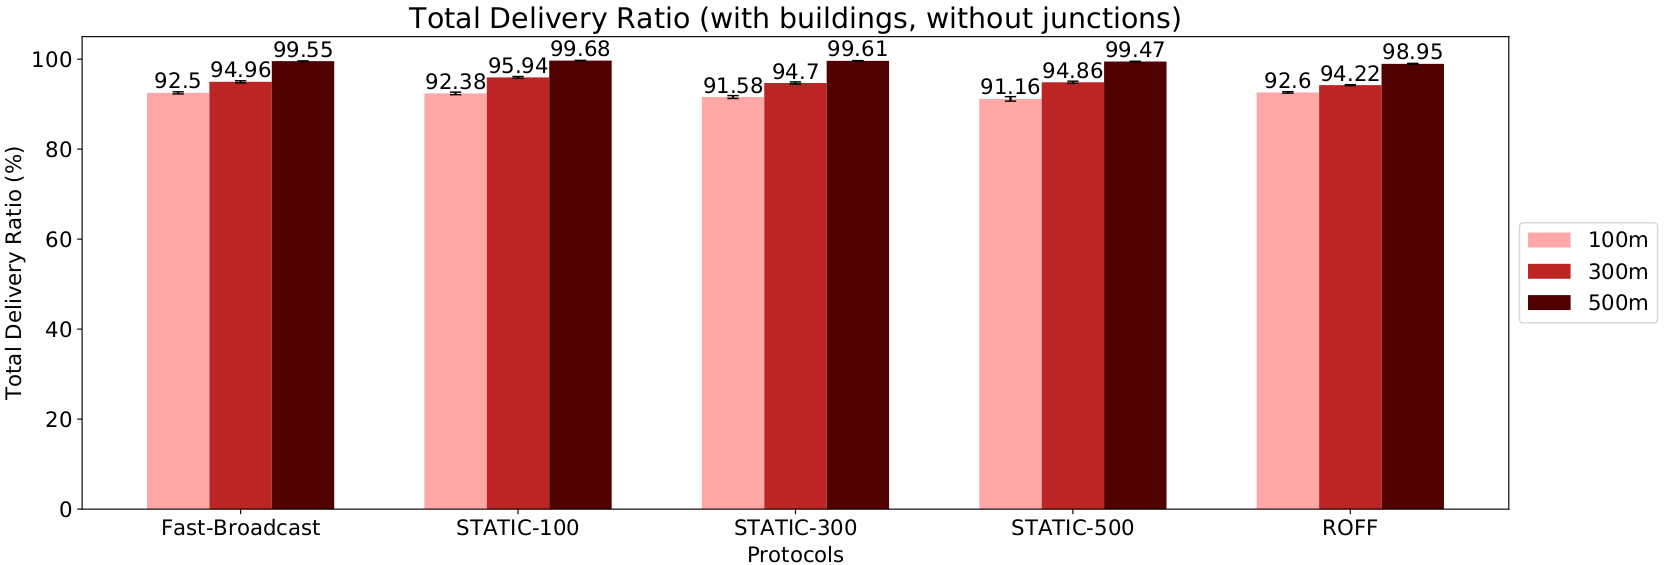
\includegraphics[width=1.0\textwidth]{immagini/la-25/b1/j0/tdr}
			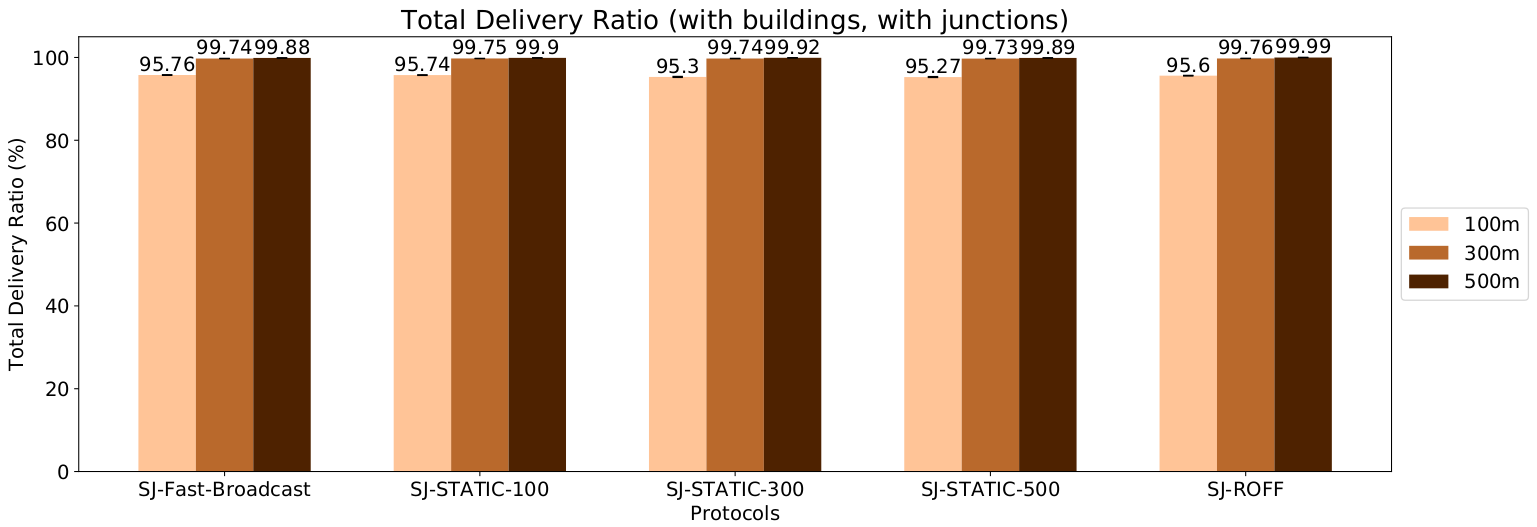
\includegraphics[width=1.0\textwidth]{immagini/la-25/b1/j1/tdr}
			\caption{\textit{TDR} for Los Angeles urban scenario}
			\label{fig:la-25-tdr}
		\end{figure}
	
		\begin{figure}[H]
			\centering
			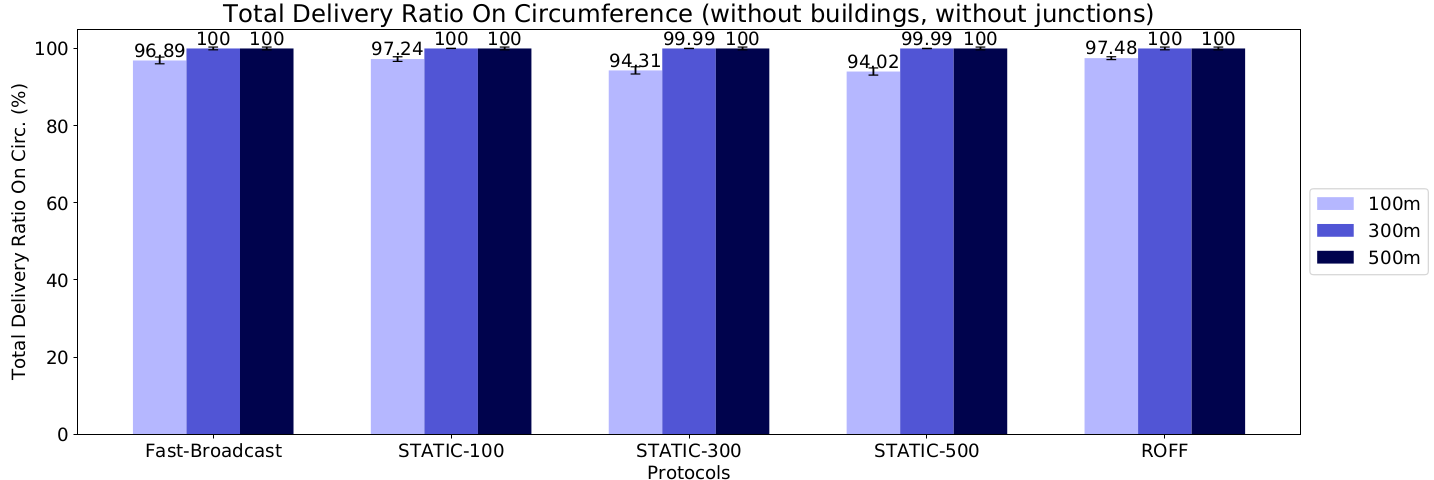
\includegraphics[width=1.0\textwidth]{immagini/la-25/b0/j0/tdroc}
			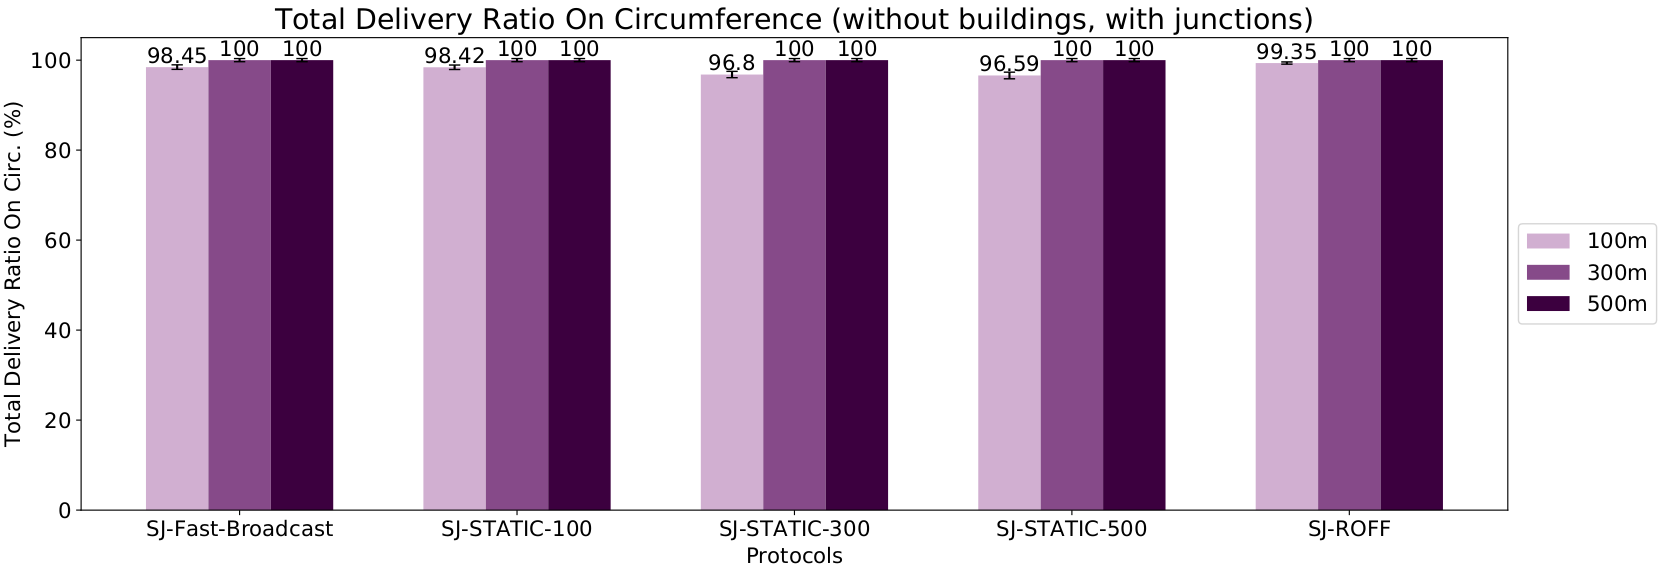
\includegraphics[width=1.0\textwidth]{immagini/la-25/b0/j1/tdroc}
			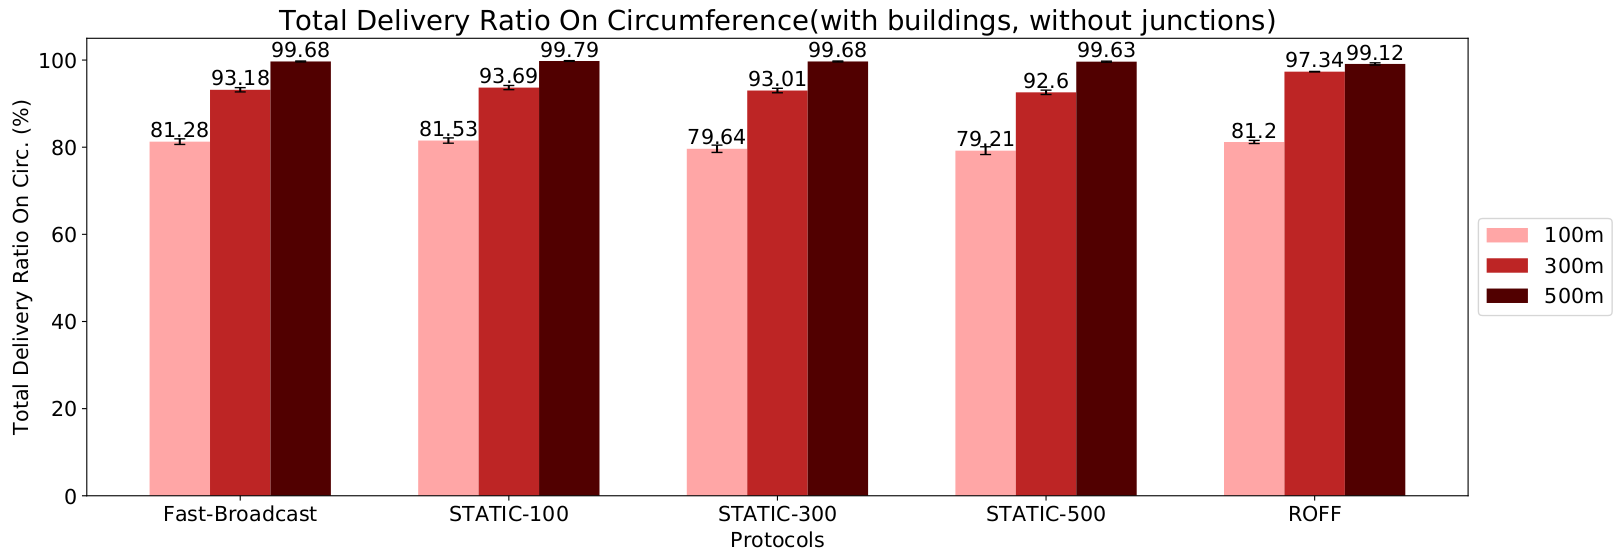
\includegraphics[width=1.0\textwidth]{immagini/la-25/b1/j0/tdroc}
			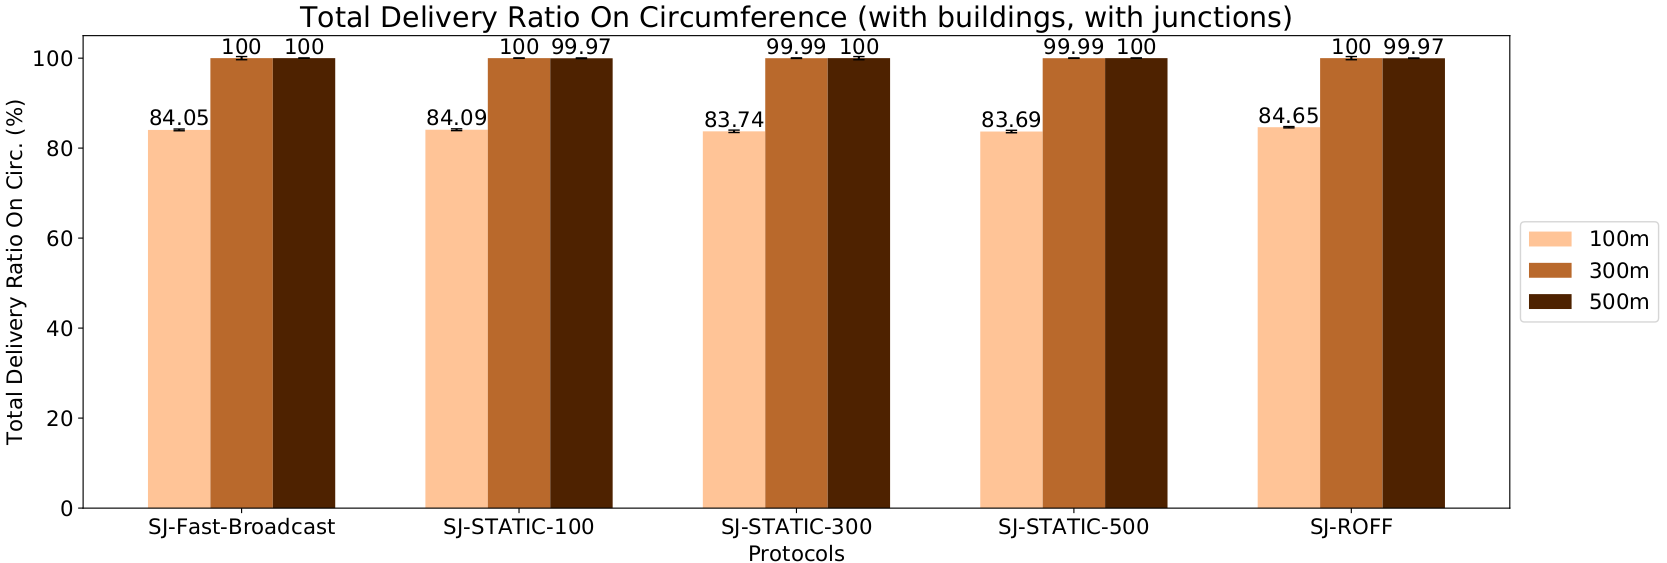
\includegraphics[width=1.0\textwidth]{immagini/la-25/b1/j1/tdroc}
			\caption{\textit{TDROC} for Los Angeles urban scenario}
			\label{fig:la-25-tdroc}
		\end{figure}

		\begin{figure}[H]
			\centering
			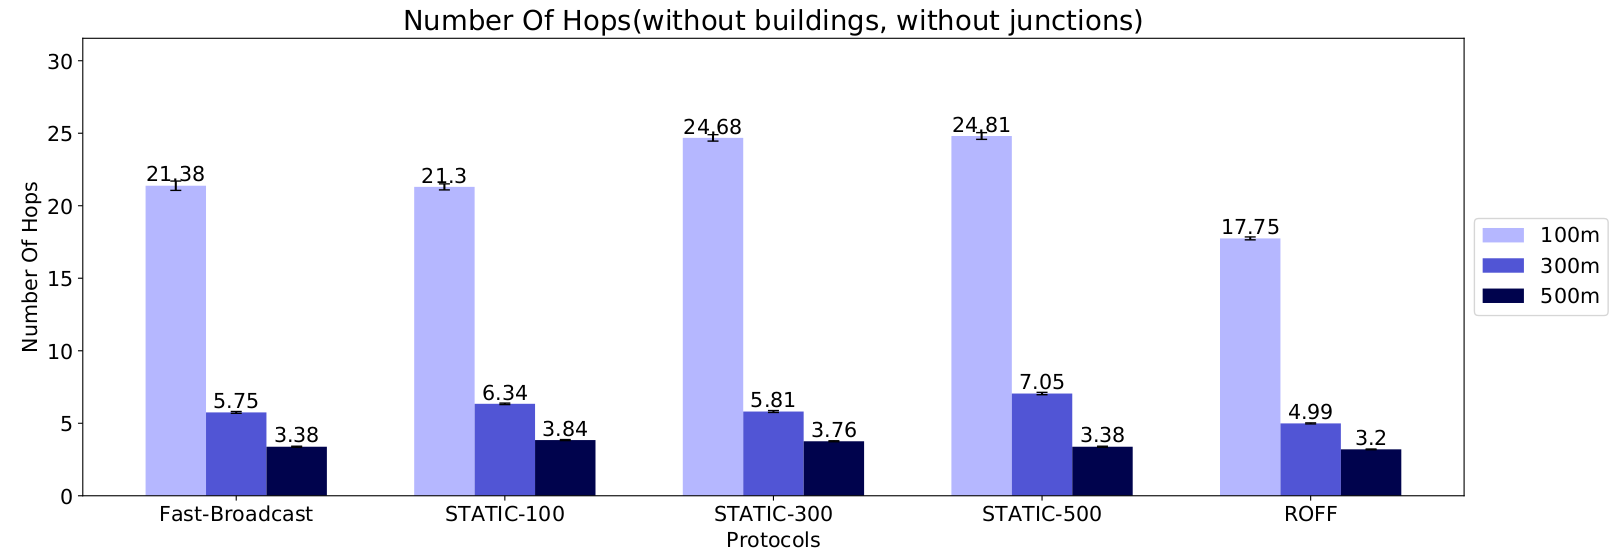
\includegraphics[width=1.0\textwidth]{immagini/la-25/b0/j0/noh}
			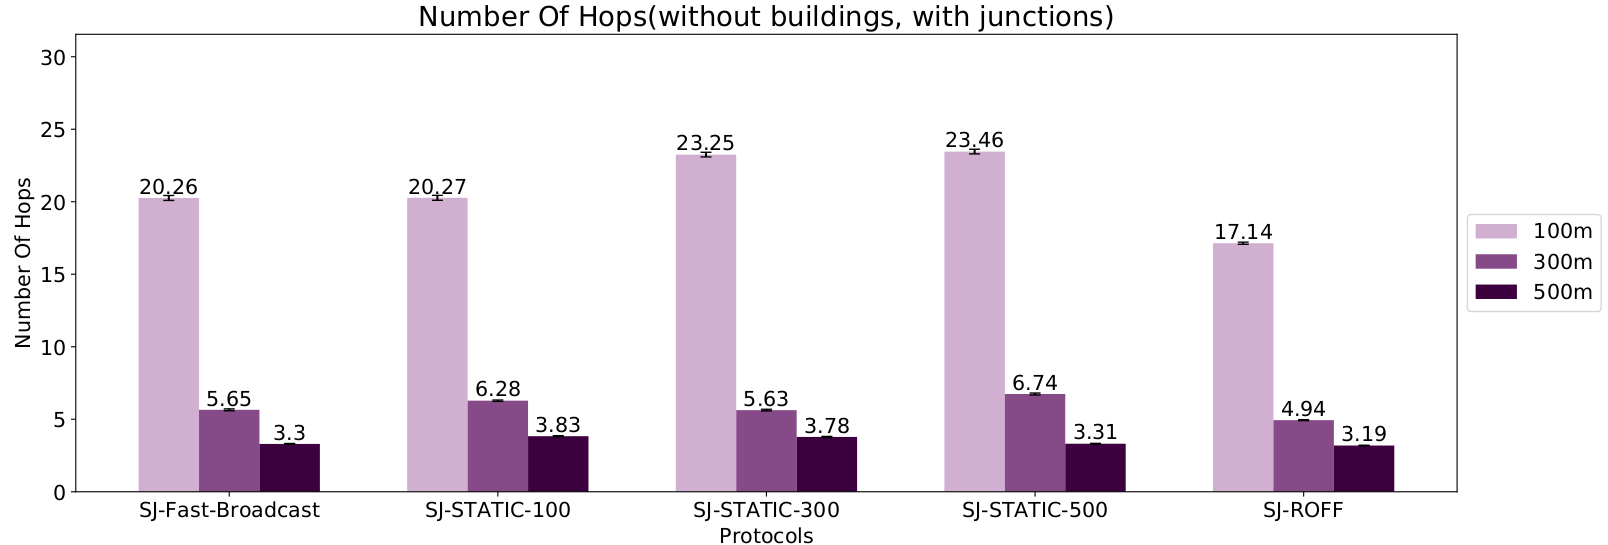
\includegraphics[width=1.0\textwidth]{immagini/la-25/b0/j1/noh}
			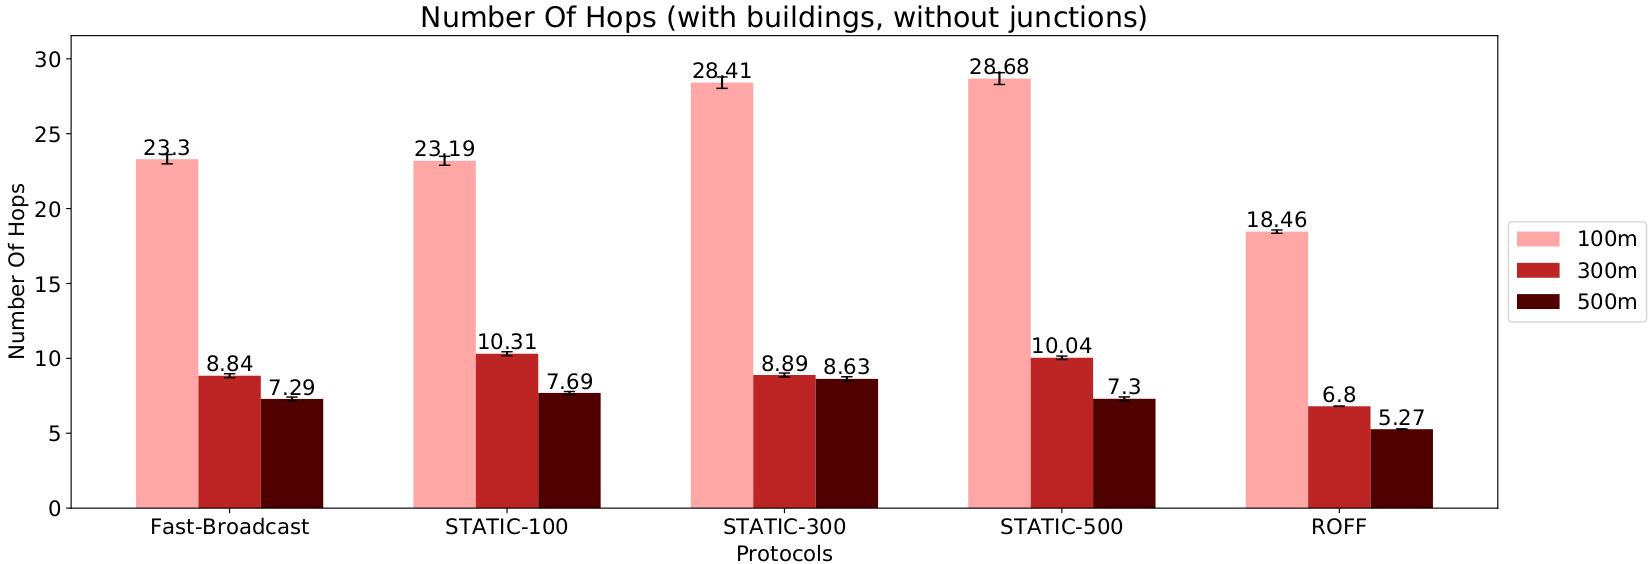
\includegraphics[width=1.0\textwidth]{immagini/la-25/b1/j0/noh}
			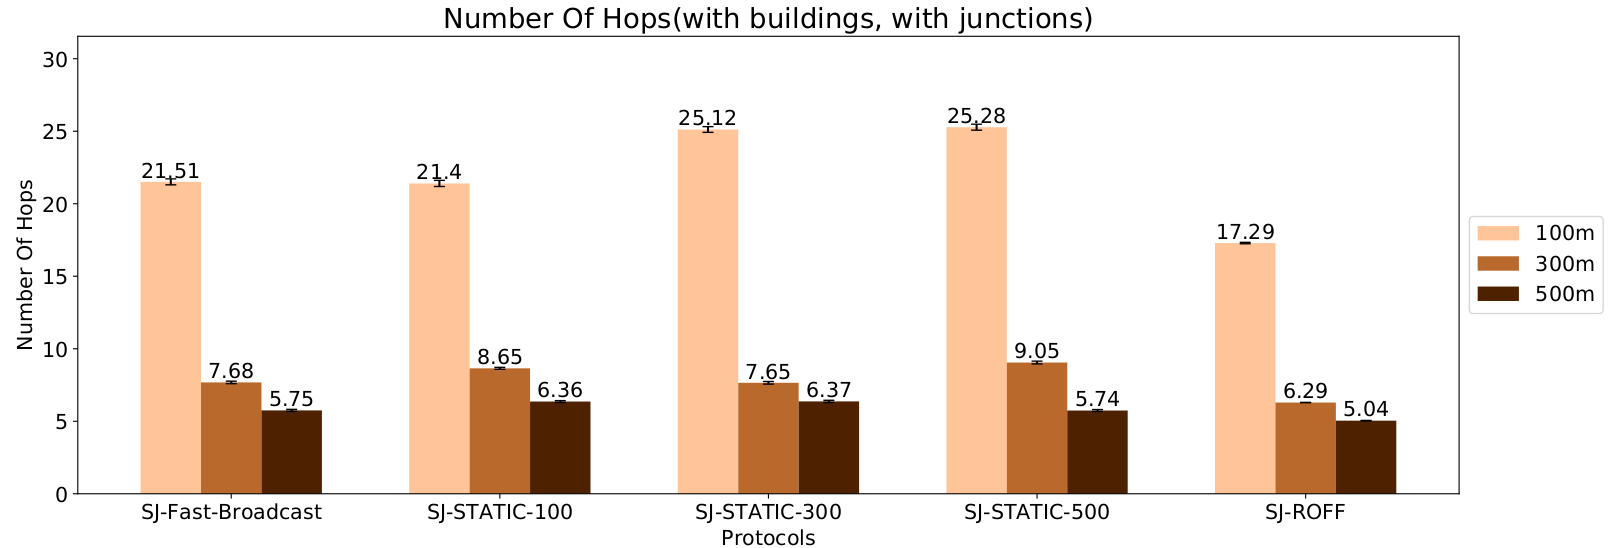
\includegraphics[width=1.0\textwidth]{immagini/la-25/b1/j1/noh}
			\caption{\textit{NOH} for Los Angeles urban scenario}
			\label{fig:la-25-noh}
		\end{figure}

		\begin{figure}[H]
			\centering
			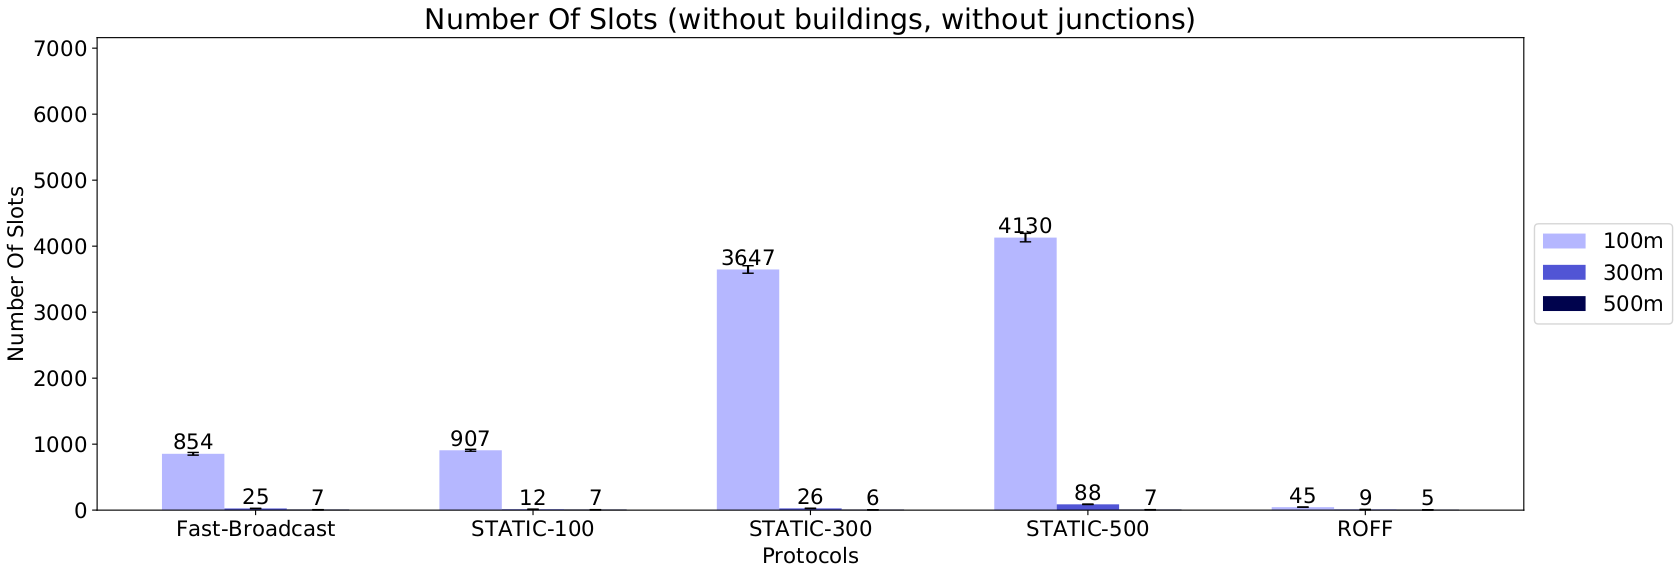
\includegraphics[width=1.0\textwidth]{immagini/la-25/b0/j0/nos}
			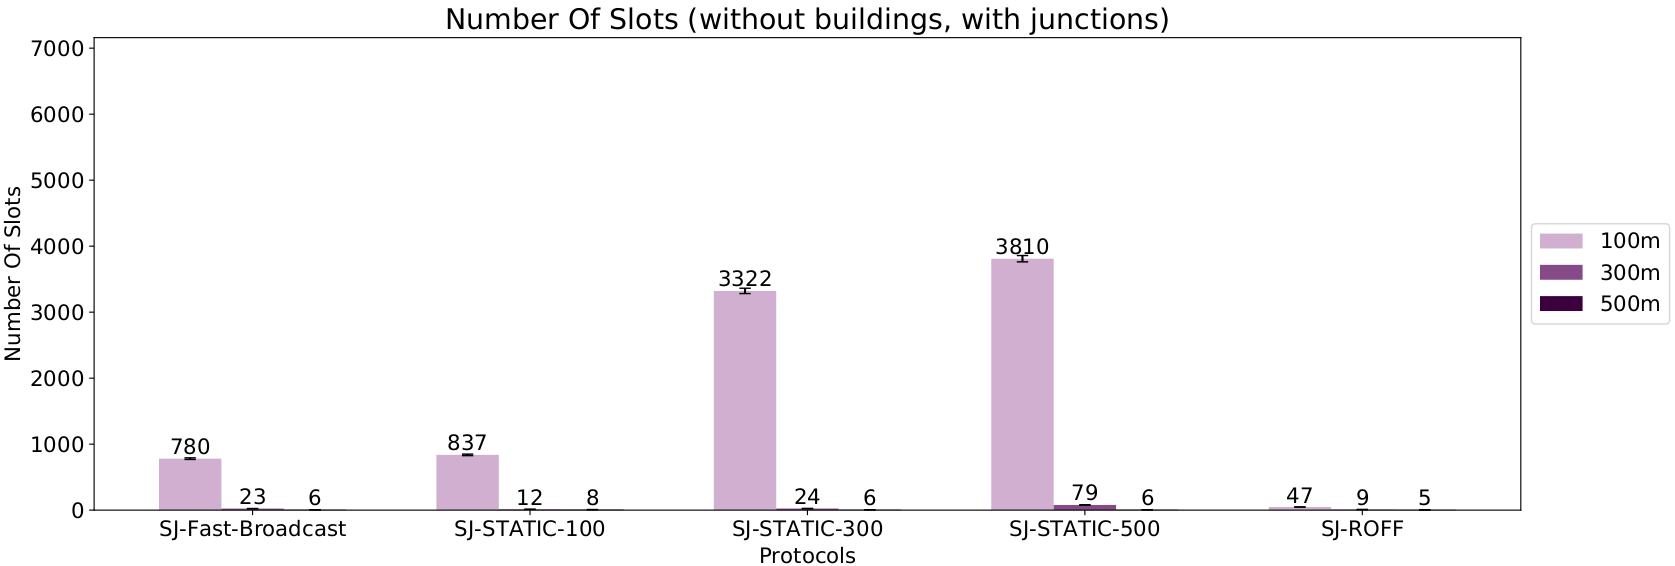
\includegraphics[width=1.0\textwidth]{immagini/la-25/b0/j1/nos}
			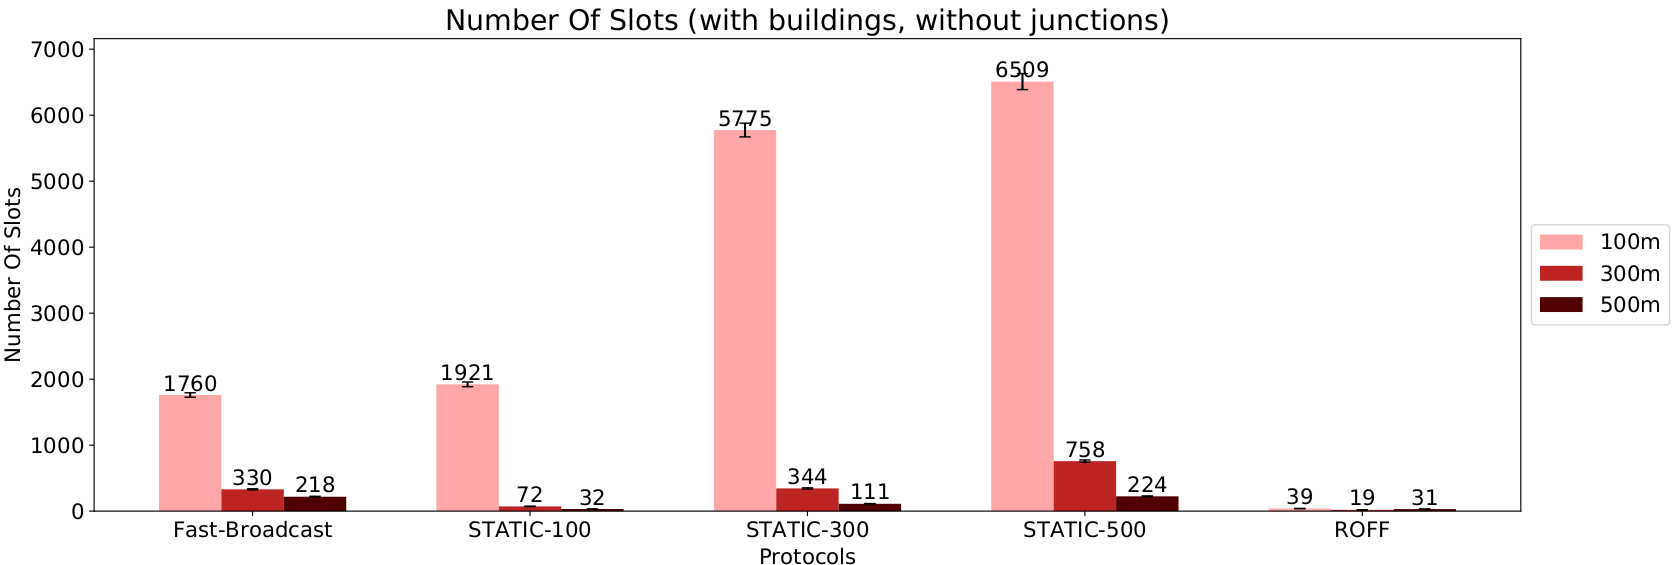
\includegraphics[width=1.0\textwidth]{immagini/la-25/b1/j0/nos}
			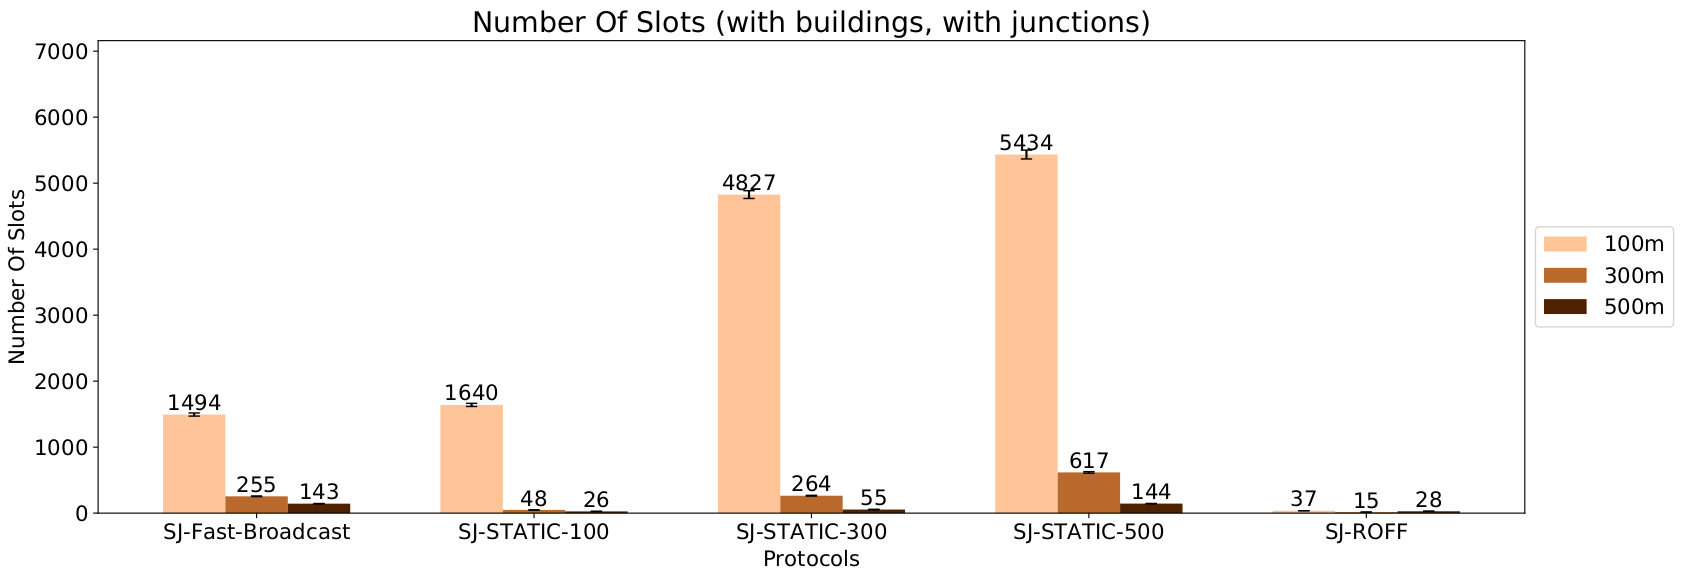
\includegraphics[width=1.0\textwidth]{immagini/la-25/b1/j1/nos}
			\caption{\textit{NOS} for Los Angeles urban scenario}
			\label{fig:la-25-nos}
		\end{figure}

		\begin{figure}[H]
			\centering
			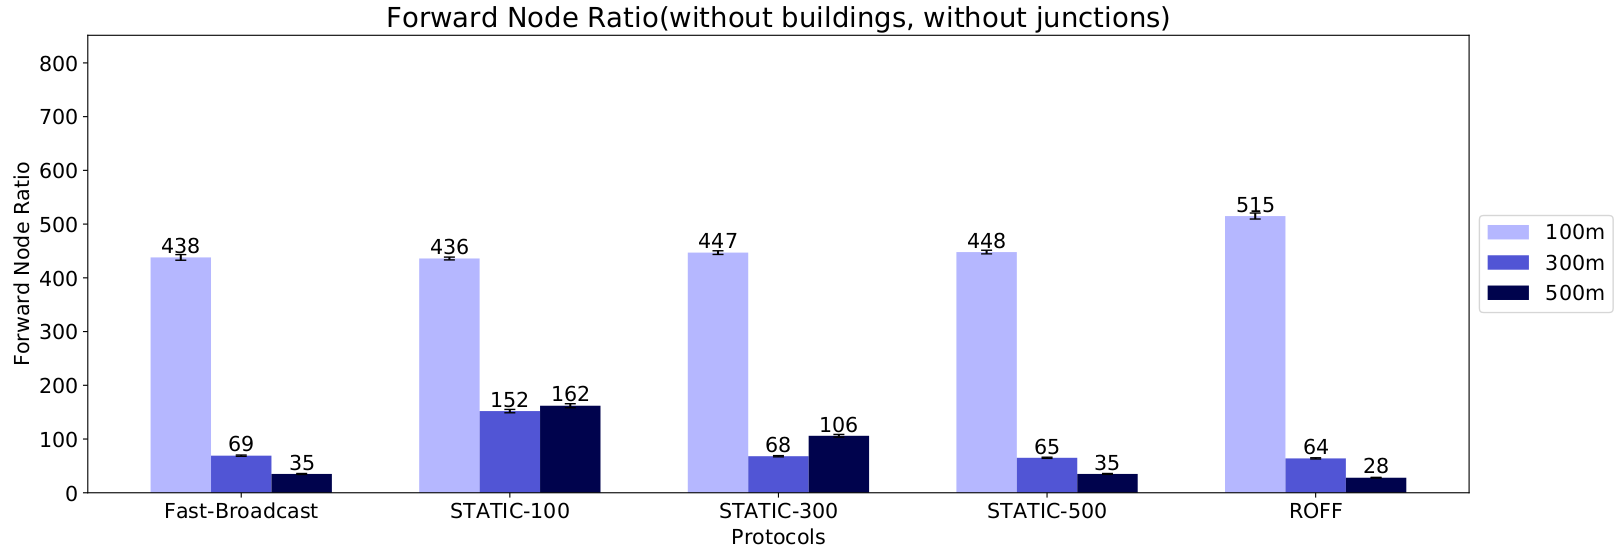
\includegraphics[width=1.0\textwidth]{immagini/la-25/b0/j0/fnn}
			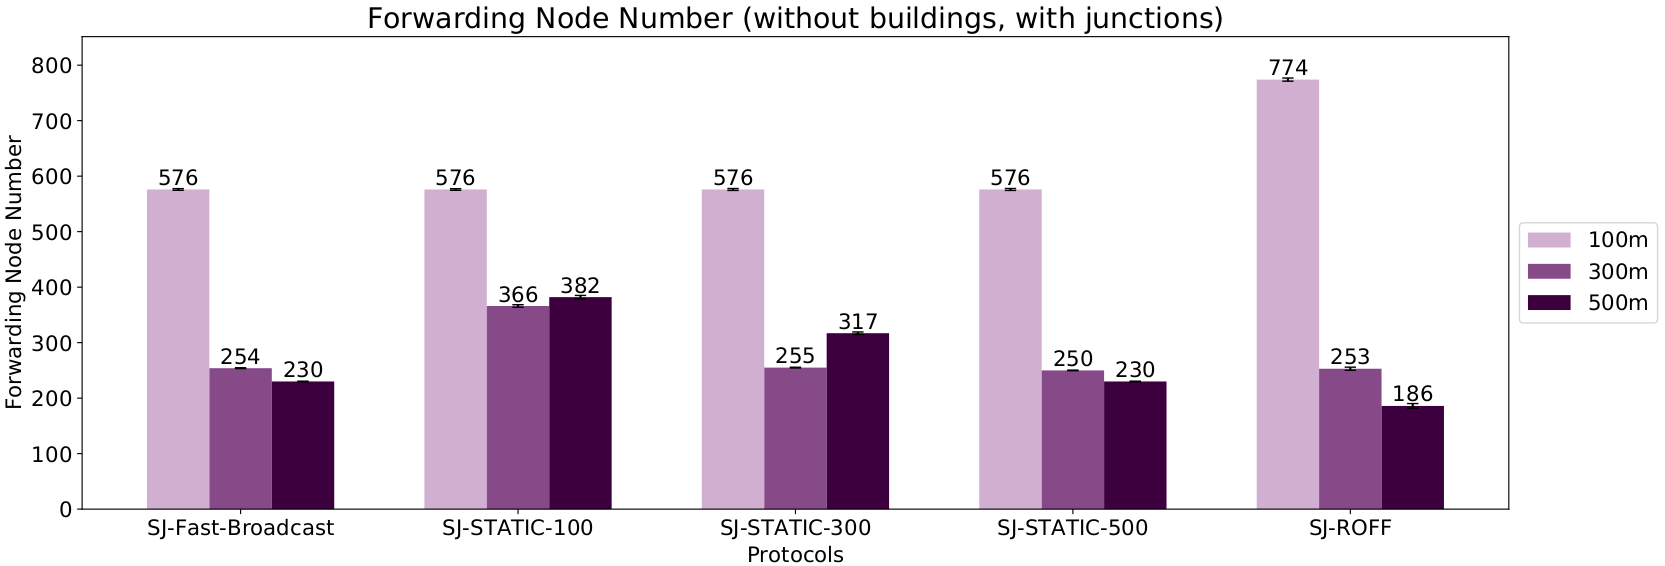
\includegraphics[width=1.0\textwidth]{immagini/la-25/b0/j1/fnn}
			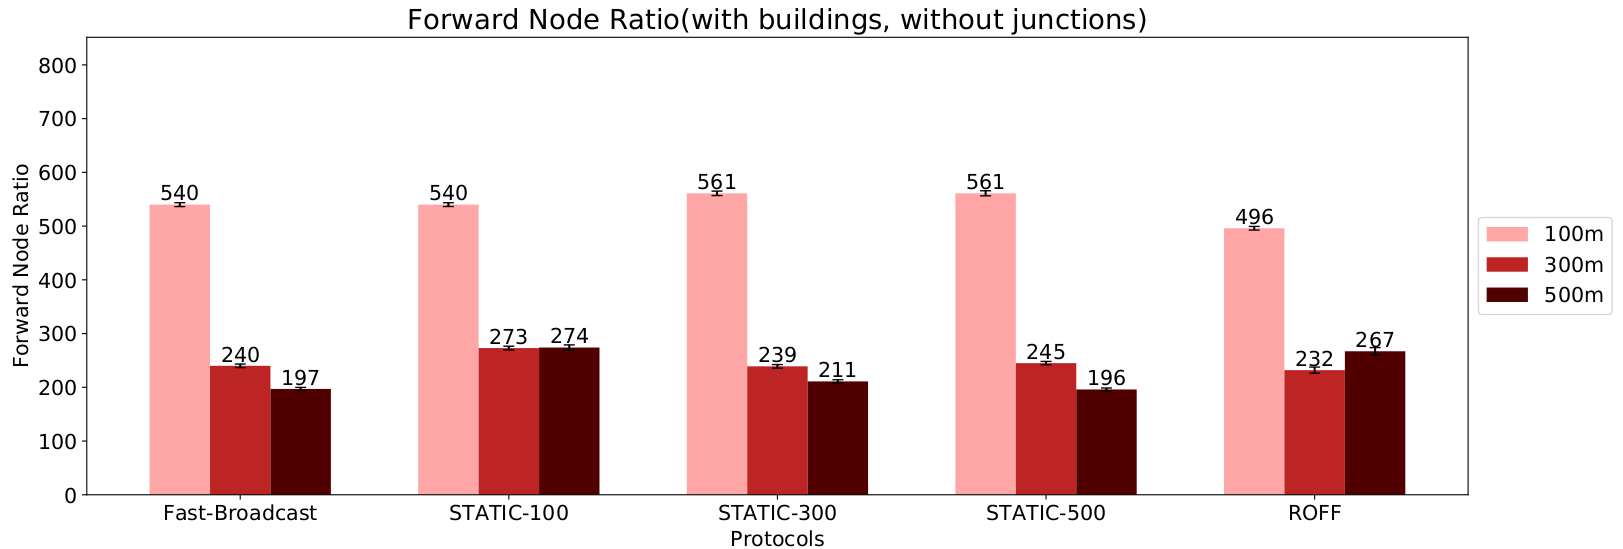
\includegraphics[width=1.0\textwidth]{immagini/la-25/b1/j0/fnn}
			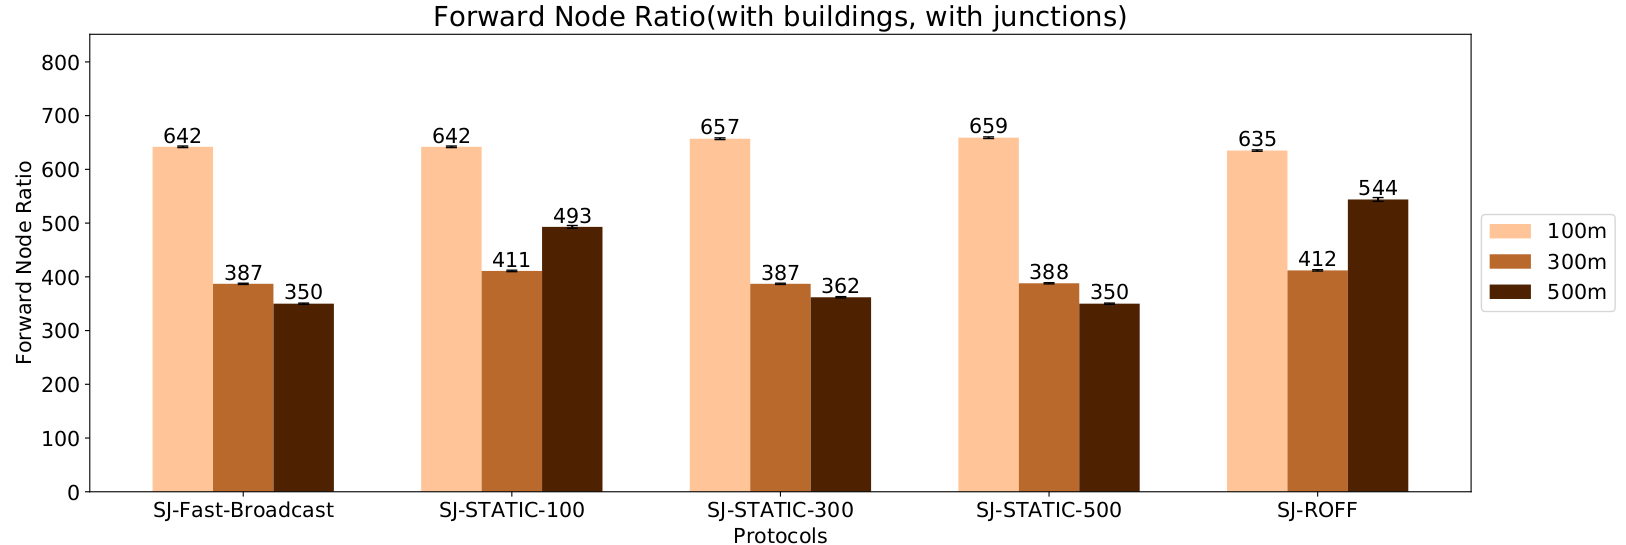
\includegraphics[width=1.0\textwidth]{immagini/la-25/b1/j1/fnn}
			\caption{\textit{FNN} for Los Angeles urban scenario}
			\label{fig:la-25-fnn}
		\end{figure}
	
		It is possible to observe the effects of the Obstacle Shadowing model on \textit{Total Delivery Ratio} and \textit{Total Delivery Ratio On Circumference}. The effects are pretty mild across all configurations, but are more noticeable with lower transmission ranges (100 and 300 meters). For example, introducing the shadowing model without considering junctions leads to a decrease of 5.97\% (98.38 to 92.5) in \textit{TDR} (Figure \ref{fig:la-25-tdr}) with a transmission range of 100 meters and a decrease of 5\% (99.96 to 94.96) with transmission range of 300 meters for Fast-Broadcast. Results for ROFF are comparable, with decreases of 6.28\% and 5.73\% respectively.
		
		
		The decrease in \textit{TDROC} (Figure \ref{fig:la-25-tdr}) is much more noticeable, especially for the 100 meters transmission range. The value decrease by 16.11\% for Fast-Broadcast and 16.74\% for ROFF. This means that introducing building shadowing leads to more problems when the Alert Message has to reach farther distances. This phenomenon can be seen in Figure \ref{fig:la-coverage-fb100}.
		Vehicles not reached by the Alert Message are more concentrated towards the circumference instead of the center.
		
		\begin{figure}[H]
			\centering
			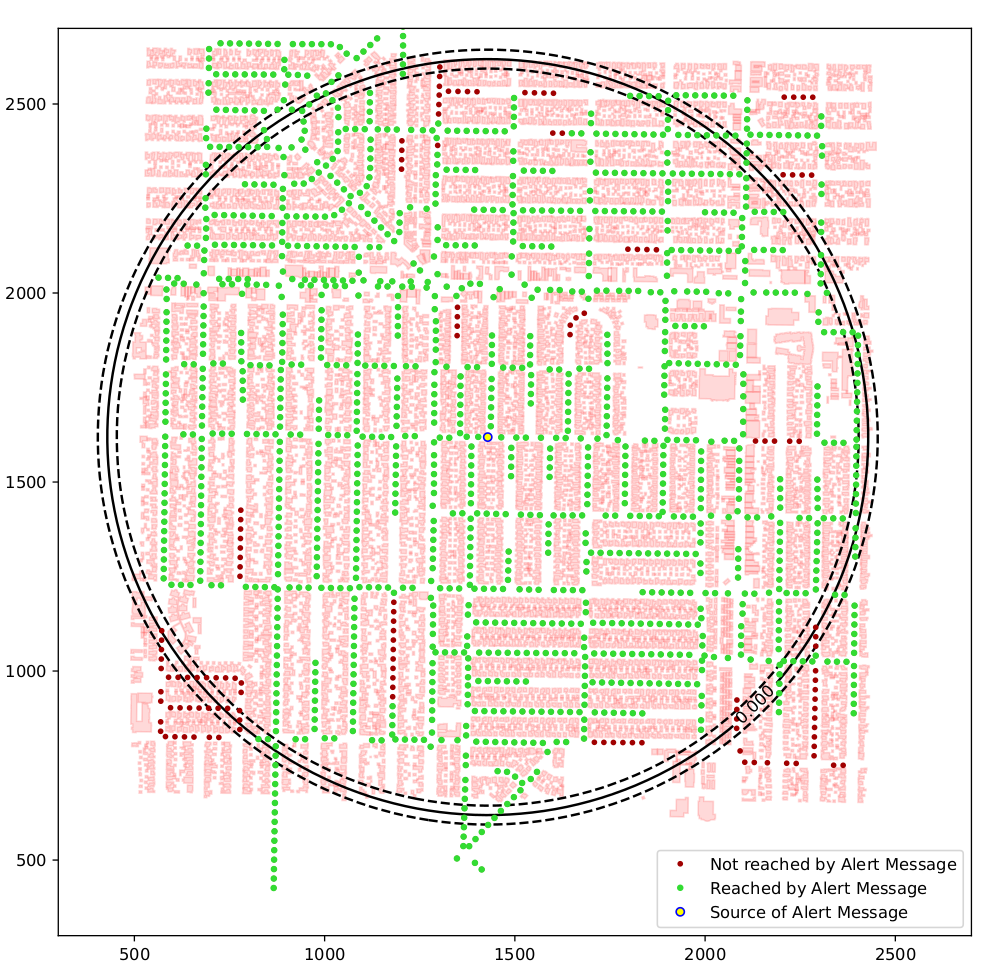
\includegraphics[width=1.0\textwidth]{immagini/la-25/la-coverage-fb100}
			\caption{Alert Message delivery for Los Angeles scenario with buildings and without junctions (Fast-Broadcast with 100 meters transmission range)}
			\label{fig:la-coverage-fb100}
		\end{figure}
		
		The introduction of the smart junction variants of the algorithms proves to be fairly effective, increasing \textit{TDR} by 3,52\% and 5,03\% when employing SJ-Fast-Broadcast instead of Fast-Broadcast for the scenario with buildings and transmission range of 100 and 300 meters respectively. Increases of the same magnitude can be noticed when utilizing SJ-ROFF instead of ROFF. With regards to \textit{TDROC}, both SJ-Fast-Broadcast and SJ-ROFF reach 100\% for 300 and 500 meters transmission ranges, while having a mild increase of around 3,40\% for 100 meters transmission range.
		
		
		Considering the Number Of Hops to reach the circumference (Figure \ref{fig:la-25-noh}), we can observe that the introduction of the shadowing model leads to an increase in the metric's value across all algorithms. Comparing the first and third configuration, \textit{NOH} rises by 8.98\%, 53.74\% and 115.68\% for Fast-Broadcast, and by 3.85\%, 36.27\% and 64.69\% for ROFF, for the three increasing transmission ranges. We notice that:
		\begin{enumerate}
			\item the rise increases with the increase in transmission range;
			\item Fast-Broadcast is affected in a greater way by the shadowing model compared to ROFF.
		\end{enumerate}
		The first point is expected, since the one-hop progress is greater in a scenario with a higher transmission range. This leads to a greater probability for the signal to run into a building. In a scenario with a lower transmission range, transmissions have a lower probability to run into a building and follow more closely the road segment even without the effects of buildings. Hence, they are less likely to be influenced by the model. The second point may be due to the fact ROFF's Neighbor Table mechanism continues to work well to identify the FFC along the road segment, leading to a smaller increase in the number of hops.
		
		
		SJ-Fast-Broadcast and SJ-ROFF need less hops in order to reach the circumference than their counterparts which do not take junctions into consideration. This holds true for both scenarios with and without buildings. This is probably due to the additional transmissions inside junctions, which help to propagate the signal along road segments in a linear way, hence covering more space with each hop. SJ-ROFF performs better than SJ-Fast-Broadcast with regards to \textit{NOH}. The difference between the two algorithms decreases as the transmission range increases.
		
		
		Regarding \textit{NOS} (Figure \ref{fig:la-25-nos}), Fast-Broadcast results increase by 106.09\%, 1220\% and 3014\% while ROFF's ones increase by 111.11\% and 520\% for 300 and 500 meters transmission range, and decrease by 4.44\% for 100 meters transmission range, when going from a building-less scenario to a scenario with buildings. Moreover, Fast-Broadcast's values are 4412.82\%, 1636.84\% and 603.23\% higher than ROFF's values in the scenario with buildings. This goes to show the effect of empty space distribution on waiting times (here represented by the number of slots waited): when the distance between the FFC and the previous forwarder is close to the estimated transmission range, then Fast-Broadcast's waiting slots are pretty close to the minimum. But when obstacles are introduced, there might not be any PFC whose distance is close to the estimated transmission range. Hence, the FFC will wait a very long time. ROFF is not affected by this phenomenon thanks to the forwarding priority acquisition, as introduced in Chapter \ref{chapter:roff}. Comparing the third and fourth image in Figure \ref{fig:la-25-nos}, we can see that the introduction of junctions is beneficial for both algorithms, leading to a decrease in \textit{NOS}. This is a consequence of the abovementioned decrease in Number Of Hops.
			
		Concerning the Forwarding Node Number (Figure \ref{fig:la-25-fnn}), the value increases when the shadowing model is introduced. ROFF with 100 meters transmission range is the only configuration where the values decreases. This configuration needs further testing in order to be explained.
		The introduction of junctions brings about an increase in the number of forwardings for all algorithms, as expected. Focusing on the fourth image of Figure \ref{fig:la-25-fnn}, SJ-ROFF is affected greatly by this increase, almost equalling SJ-Fast-Broadcast with 100 meters transmission range, and with much greater \textit{FNN} values in 300 and 500 meters transmission range configurations. This might be caused by the introduction of transmissions inside junctions, which exacerbate the collision problem already reported in the previous section (Figure \ref{fig:2d-roff}), leading to an imperfect suppression of scheduled transmissions. The problem is not as severe as in the Grid scenario since the node distribution is less regular, but overall Fast-Broadcast performs better than ROFF in terms of \textit{FNN}.
	
	\section{Padua urban scenario}
		\label{sec:padua-urban}
		As reported in the previous section the Los Angeles scenario, despite being realistic, still had a certain degree of regularity for what concerns vehicle distribution and scenario topology. In fact, roads and sidewalks are pretty large and the overall road positioning resembles a Grid scenario. The next step in testing consisted in employing the algorithms in a more difficult scenario, with narrower roads and intersections, smaller (if any) sidewalks and pedestrian zones where no traffic is allowed. The chosen scenario is located in Padua and, as the previous one, data about the scenario have been retrieved by OSM and processed through SUMO. The scenario is depicted in Figure \ref{fig:padua-scenario}, while its configuration is reported in Table \ref{tab:padua-25}. 
		
		\begin{figure}[H]
			\centering
			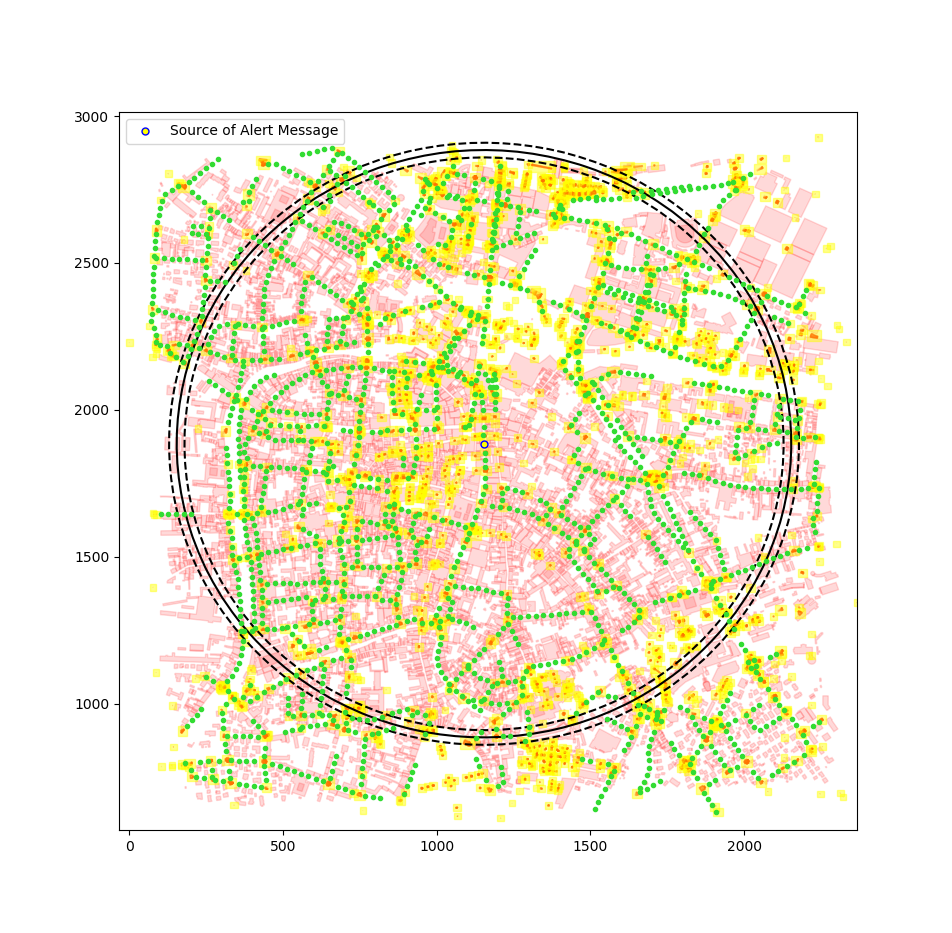
\includegraphics[width=0.98\textwidth]{immagini/padua-25/padua-scenario}
			\caption{Padua urban scenario depiction}
			\label{fig:padua-scenario}
		\end{figure}
	
		\begin{table}[H]
			\def\arraystretch{1.1}
			\rowcolors{2}{D}{P}	
			\begin{tabularx}{\textwidth}{l | l  l}
				\rowcolor{I} {\large \textcolor{white}{Parameter}} & {\large \textcolor{white}{Value}} & {\large \textcolor{white}{}} \TBstrut  \\
				\toprule
				\endhead
				%			\midrule[1pt]
				\rowcolor{P} \multicolumn{3}{c}{Scenario configuration} \\
				\midrule[1pt]
				Latitude N								& 45.4171				& \textdegree		\\
				Latitude S								& 45.3981				& \textdegree		\\
				Longitude W								& 11.8654				& \textdegree		\\
				Longitude E								& 11.8923				& \textdegree		\\
				Road length 							& 1200	 				& m		\\
				Distance between vehicles 				& 25					& m		\\
				Circumference radius					& 1000					& m		\\
				Number of vehicles						& 1775					& 		\\
				Source of alert message position		& Center				&		\\
				Number of buildings						& 6322					&		\\
				Number of junctions						& 3231					&		\\	
				\midrule[1pt]
				\rowcolor{P} \multicolumn{3}{c}{Simulator configuration} \\
				\midrule[1pt]
				Shadowing model							& Obstacle Shadowing 	&		\\
				Junction modeling						& Yes					&		\\
				\midrule[1pt]
				Number of simulations per configuration	& 4500					&		\\
				\bottomrule
			\end{tabularx}
			\caption{Los Angeles urban scenario configuration}
			\label{tab:padua-25}
		\end{table}
	
		\begin{figure}[H]
			\centering
			\includegraphics[width=1.0\textwidth]{immagini/padua-25/b0/j0/tdr}
			\includegraphics[width=1.0\textwidth]{immagini/padua-25/b0/j1/tdr}
			\includegraphics[width=1.0\textwidth]{immagini/padua-25/b1/j0/tdr}
			\includegraphics[width=1.0\textwidth]{immagini/padua-25/b1/j1/tdr}
			\caption{\textit{TDR} for Padua urban scenario}
			\label{fig:padua-25-tdr}
		\end{figure}
		
		\begin{figure}[H]
			\centering
			\includegraphics[width=1.0\textwidth]{immagini/padua-25/b0/j0/tdroc}
			\includegraphics[width=1.0\textwidth]{immagini/padua-25/b0/j1/tdroc}
			\includegraphics[width=1.0\textwidth]{immagini/padua-25/b1/j0/tdroc}
			\includegraphics[width=1.0\textwidth]{immagini/padua-25/b1/j1/tdroc}
			\caption{\textit{TDROC} for Padua urban scenario}
			\label{fig:padua-25-tdroc}
		\end{figure}
		
		\begin{figure}[H]
			\centering
			\includegraphics[width=1.0\textwidth]{immagini/padua-25/b0/j0/noh}
			\includegraphics[width=1.0\textwidth]{immagini/padua-25/b0/j1/noh}
			\includegraphics[width=1.0\textwidth]{immagini/padua-25/b1/j0/noh}
			\includegraphics[width=1.0\textwidth]{immagini/padua-25/b1/j1/noh}
			\caption{\textit{NOH} for Padua urban scenario}
			\label{fig:padua-25-noh}
		\end{figure}
		
		\begin{figure}[H]
			\centering
			\includegraphics[width=1.0\textwidth]{immagini/padua-25/b0/j0/nos}
			\includegraphics[width=1.0\textwidth]{immagini/padua-25/b0/j1/nos}
			\includegraphics[width=1.0\textwidth]{immagini/padua-25/b1/j0/nos}
			\includegraphics[width=1.0\textwidth]{immagini/padua-25/b1/j1/nos}
			\caption{\textit{NOS} for Padua urban scenario}
			\label{fig:padua-25-nos}
		\end{figure}
		
		\begin{figure}[H]
			\centering
			\includegraphics[width=1.0\textwidth]{immagini/padua-25/b0/j0/fnn}
			\includegraphics[width=1.0\textwidth]{immagini/padua-25/b0/j1/fnn}
			\includegraphics[width=1.0\textwidth]{immagini/padua-25/b1/j0/fnn}
			\includegraphics[width=1.0\textwidth]{immagini/padua-25/b1/j1/fnn}
			\caption{\textit{FNN} for Padua urban scenario}
			\label{fig:padua-25-fnn}
		\end{figure}
	
		In this scenario the effects of obstacle shadowing on delivery ratios is quite large, especially for the 300 and 500 meters cases, for all algorithms. We have a decrease in \textit{TDR} (Figure \ref{fig:padua-25-tdr}) of around 65\% for Fast-Broadcast in both transmission ranges when introducing buildings (first and third images), which results in quite poor performances. The Smart Junction variants of Fast-Broadcast manages to reach pretty good results in Total Delivery Ratio (fourth image), with 72.1\% and 91.42\% for the two transmission ranges. ROFF's results are even worse before the introduction of junctions, with \textit{TDR} below 10\% for the lowest transmission range. Even in this case, SJ-ROFF manages to improve the values, slightly overcoming SJ-Fast-Broadcast's results.
		
		
		The same observations hold true even for \textit{TDROC} (Figure 	\ref{fig:padua-25-tdr}). Hence, the benefits of junctions are twofold even for this scenario regarding delivery ratios.
		
		
		Concerning \textit{NOS}, the increase due to the obstacle model is even more pronounced than the previous scenario for both algorithms. Due to the lower coverage, it is possible that the few messages which reach the circumference go through a very irregular path and  one-hop progress is quite low. The introduction of junctions, as in the Los Angeles scenario, causes a decrease in \textit{NOH}. One anomalous results is ROFF with 100 meters transmission range, whose values shoots up by more than 232\% when comparing it with SJ-ROFF, and is much higher than SJ-Fast-Broadcast under the same conditions. This phenomenon might be due to the harsher vehicle distribution, obstacle and junction positioning which cause the signal to follow very long paths from the source to the circumference. With the other two transmission ranges, SJ-ROFF outperforms SJ-Fast-Broadcast.
		
		
		Results for \textit{NOH} and \textit{FNN} are comparable with the ones observed in previous scenarios.
		
		
	\section{Los Angeles smart city scenario}
		After the comparison of the algorithms in 2D scenarios, we wanted to test them in a mixed 2D-3D scenario, where drones were also employed. Drones are utilized in many military and civil applications, such as agriculture, environmental protection and traffic flow control. It is foreseeable that they will also be a part of the development of the so called \jquote{smart cities}, defined as \jquote{the use of discrete new technology applications such as RFID and Internet Of Things through more holistic conception of intelligent, integrated working that is closely linked to the concept of living and user generated services}\cite{smartCity}. One of the possible applications of drones in a urban scenario could make them help vehicles in Emergency Message Dissemination in order to exploit their greater field of view and bypass the effects of ground level shadowing and obstacles. 
		
		
		This scenario is built upon the Los Angeles urban scenario presented in Section \ref{sec:la-scenario}. Two layers of drones were added to the ground level of vehicles: 
		\begin{itemize}
			\item the first layer is situated at a height of 30 meters from ground level and employs 732 drones;
			\item the second layer, employing the same number of drones, is situated at a height of 60 meters.
		\end{itemize}
		Drones are more spaced from one another than vehicles, with an average distance of 50 meters. We also wanted to test the effects of the Obstacle Model on drones in this scenario. Since the maximum height of a building in the data retrieved from OpenStreetMap is 21.9 meters, drones would not have their line of sight affected by the obstacles. Hence, as an additional configuration of this scenario, all buildings have been heightened to be taller than the second layer of drones (e.g. every building is high 100 meters). 
		
		
		One important fact to notice is that, even if we have called the object placed inside the two layers \jquote{drones}, this scenario applies also if those objects were other kinds of network connected entities, such as customers' access points or IoT devices.
		
		Figure \ref{fig:la-smart-city} shows a representation of the two scenarios with buildings.
		
		\begin{figure}[H]
			\centering
			\includegraphics[width=0.95\textwidth]{immagini/la-smart-city-low}
			\includegraphics[width=0.95\textwidth]{immagini/la-smart-city-high}
			\caption{Los Angeles smart city scenario with real height buildings (top) and very high buildings (bottom)}
			\label{fig:la-smart-city}
		\end{figure}
		\newpage
		
		In this scenario, the \textit{TDR} metric considers delivery to all entities in the scenario (both vehicles and drones), while the circumference relative to the area of interest continues to be defined in the same way as the 2D Los Angeles urban scenario, hence \textit{TDROC} concerns exclusively vehicles.
		
		
		All configurations are reported in Figure \ref{fig:la-smart-city-overview}, whose colors will guide the following graph results. Table \ref{tab:la-smart-city} reports all the scenario settings.
		
		\begin{figure}[H]
			\centering
			\includegraphics[width=0.7\textwidth]{immagini/la-smart-city/overview}
			\caption{Test overview of Los Angeles smart city scenario}
			\label{fig:la-smart-city-overview}
		\end{figure}
		
	\begin{table}[H]
		\def\arraystretch{1.1}
		\rowcolors{2}{D}{P}	
		\begin{tabularx}{\textwidth}{l | l  l}
			\rowcolor{I} {\large \textcolor{white}{Parameter}} & {\large \textcolor{white}{Value}} & {\large \textcolor{white}{}} \TBstrut  \\
			\toprule
			\endhead
			%			\midrule[1pt]
			\rowcolor{P} \multicolumn{3}{c}{Scenario configuration} \\
			\midrule[1pt]
			Circumference radius					& 1000					& m		\\
			Number of vehicles						& 1465					& 		\\
			Distance between vehicles 				& 25					& m		\\
			Source of alert message position		& Center				&		\\
			Number of drone layers					& 2						&		\\
			Height of first drone layer				& 30					& m		\\
			Number of drones in first layer			& 732					& 		\\
			Height of second drone layer			& 60					& m		\\
			Number of drones in second layer		& 732					& 		\\
			Distance between drones (average)		& 50					& m		\\
			Number of buildings						& 8241					&		\\
			Building heights						& Real, 100				& m		\\
			\midrule[1pt]
			\rowcolor{P} \multicolumn{3}{c}{Simulator configuration} \\
			\midrule[1pt]
			Shadowing model							& Obstacle Shadowing 	&		\\
			Junction modeling						& No					&		\\
			\midrule[1pt]
			Number of simulations per configuration	& 1000					&		\\
			\bottomrule
		\end{tabularx}
		\caption{Los Angeles urban scenario configuration}
		\label{tab:la-smart-city}
	\end{table}

	\begin{figure}[H]
		\centering
		\includegraphics[width=1.0\textwidth]{immagini/la-smart-city/b0/tdr}
		\includegraphics[width=1.0\textwidth]{immagini/la-smart-city/b1/h0/tdr}
		\includegraphics[width=1.0\textwidth]{immagini/la-smart-city/b1//h1/tdr}
		\caption{\textit{TDR} for Los angeles smart city scenario}
		\label{fig:la-smart-city-tdr}
	\end{figure}

	\begin{figure}[H]
		\centering
		\includegraphics[width=1.0\textwidth]{immagini/la-smart-city/b0/tdroc}
		\includegraphics[width=1.0\textwidth]{immagini/la-smart-city/b1/h0/tdroc}
		\includegraphics[width=1.0\textwidth]{immagini/la-smart-city/b1//h1/tdroc}
		\caption{\textit{TDROC} for Los angeles smart city scenario}
		\label{fig:la-smart-city-tdroc}
	\end{figure}
	
	\begin{figure}[H]
		\centering
		\includegraphics[width=1.0\textwidth]{immagini/la-smart-city/b0/noh}
		\includegraphics[width=1.0\textwidth]{immagini/la-smart-city/b1/h0/noh}
		\includegraphics[width=1.0\textwidth]{immagini/la-smart-city/b1//h1/noh}
		\caption{\textit{NOH} for Los angeles smart city scenario}
		\label{fig:la-smart-city-noh}
	\end{figure}

	\begin{figure}[H]
		\centering
		\includegraphics[width=1.0\textwidth]{immagini/la-smart-city/b0/nos}
		\includegraphics[width=1.0\textwidth]{immagini/la-smart-city/b1/h0/nos}
		\includegraphics[width=1.0\textwidth]{immagini/la-smart-city/b1//h1/nos}
		\caption{\textit{NOS} for Los angeles smart city scenario}
		\label{fig:la-smart-city-nos}
	\end{figure}

	\begin{figure}[H]
		\centering
		\includegraphics[width=1.0\textwidth]{immagini/la-smart-city/b0/fnn}
		\includegraphics[width=1.0\textwidth]{immagini/la-smart-city/b1/h0/fnn}
		\includegraphics[width=1.0\textwidth]{immagini/la-smart-city/b1//h1/fnn}
		\caption{\textit{FNN} for Los angeles smart city scenario}
		\label{fig:la-smart-city-fnn}
	\end{figure}

	Judging by the results shown in Figure \ref{fig:la-smart-city-tdr} and \ref{fig:la-smart-city-tdroc}, drones seem to help a lot in signal propagation thanks to their altitude. In fact, the scenario without buildings and with real-height buildings yield comparable results. In the third scenario, when the obstacles's heights exceed the second drone layer's height, the shadowing effect is more pronounced for lower transmission range configurations. Overall the total delivery ratio is still acceptable, with neither Fast-Broadcast or ROFF falling under 90\%. \textit{TDROC} in configurations with 100 meters transmission range is affected in a greater way. In fact, as specified above, in this scenario the \textit{TDROC} metric is only about vehicles on the ground, so the greater shadowing due to high buildings yields the expected results.
	
	
	The effects of obstacles on \textit{NOH} (Figure \ref{fig:la-smart-city-noh}) are consistent with those observed in previous scenarios. The metric's value further increases with high buildings, since the signal probably propagates more often on the ground instead of covering larger distances thanks to inter-street drone to vehicle communications. With high buildings the propagation is restrained inside the road, hence the effects of drones are much more limited.
	
	
	Concerning \textit{NOS} (Figure \ref{fig:la-smart-city-nos}), we can notice that the increase is much higher when going from obstacles with real heights to 100 meters high obstacles. For example, focusing on the 300 meters transmission range configuration, for Fast-Broadcast we have an increase of 64.71\% from the first to the second image and of 553.57\% from the second to the third. For ROFF those values are 27.27\% and 114.29\%. Once again, this phenomenon could be due to the same effect explained in the previous paragraph: with inter-street communication heavily impeded and the increase in \textit{NOH}, \textit{NOS} increases as a consequence.
	
	
	Focusing on the 300 and 500 meters transmission range configurations, \textit{FNN} (Figure \ref{fig:la-smart-city-fnn}) increases for Fast-Broadcast and ROFF, both when going from the first image to the second and from the second to the third. This is expected, since in both cases the shadowing effects are increased and a greater number of forwarders is necessary to cover the same area. For the 100 meters case, we can notice some anomalous results: Fast-Broadcast's value stays around the same number, while ROFF's decreases considerably in the last two scenarios. The same observation about collision areas in ROFF introduced in Section \ref{sec:grid} might explain this behaviour, but it would affect in a similar way also the 300 and 500 meters configurations. Hence, this phenomenon needs more thorough testing in order to be explained.
	
	
	Overall, the two main algorithms seem to work well even in this mixed 2D and 3D scenario, with similar advantages and disadvantages reported in previous urban scenarios.
	

	\section{Hello Message forging scenario}
		In all previous tests all entities participating in the message propagation told the truth about their position and did not try to manipulate the algorithms in order to hinder the delivery process. During our analysis we wanted to test how vulnerable the algorithms were to attacks where some malicious attacker tries to increase the end to end delay (the \textit{NOS} metric in our case). The attack consists in having a malicious node send fake Hello Messages bursts to vehicles during the Estimation Phase in order to mess with their estimations. These forged messages included fake information, mainly a wrong (overestimated) transmission range and fake IDs. We tested two different levels of severity on the attack: a low severity one, reported in Section \ref{sec:low-severity}, and a high severity one, reported in Section \ref{sec:high-severity}. Several percentages of affected vehicles (i.e. the vehicles which receive the forged Hello Message bursts) ranging from 0 to 50\% have been tested. Both tests were carried out using the Los Angeles urban scenario without the effect of the Obstacle Model. Only Fast-Broadcast and ROFF algorithms were tested.
		
		\subsection{Low severity attack} 
			In the low severity attack the effect of 150 different forged Hello Messages was tested. Each forged message reports a fake position such that the detected distances by the affected node (the receiver) ranges from 301 ($txRange + 1$) to 450 ($txRange + 150$). Parameters for this scenario are reported in Table \ref{tab:low-forging}.
			\label{sec:low-severity}
				\begin{table}[H]
				\def\arraystretch{1.1}
				\rowcolors{2}{D}{P}	
				\begin{tabularx}{\textwidth}{l | l  l}
					\rowcolor{I} {\large \textcolor{white}{Parameter}} & {\large \textcolor{white}{Value}} & {\large \textcolor{white}{}} \TBstrut  \\
					\toprule
					\endhead
					%			\midrule[1pt]
					\rowcolor{P} \multicolumn{3}{c}{Scenario configuration} \\
					\midrule[1pt]
					Vehicles affected by forging			& 0, 10, 20, 30, 40, 50 & \%	\\
					Number of forged messages				& 150					&		\\
					Forged distances						& 301, 302,...,450		&		\\
					\midrule[1pt]
					\rowcolor{P} \multicolumn{3}{c}{Simulator configuration} \\
					\midrule[1pt]
					Transmission power						& 4.6					& dBm	\\
					Transmission range						& 300					& m		\\
					Shadowing model							& No					&		\\
					Junction modeling						& No					&		\\
					\midrule[1pt]
					Number of simulations per configuration	& 1000					&		\\
					\bottomrule
				\end{tabularx}
				\caption{Low severity forging attack scenario configuration based on Los Angeles urban scenario}
				\label{tab:low-forging}
			\end{table}
			
			\begin{figure}[H]
				\centering
				\includegraphics[width=1.0\textwidth]{immagini/la-25/forging/nos-low-severity}
				\caption{\textit{NOS} for low severity forging scenario}
				\label{fig:low-forging}
			\end{figure}
					
			The hello forging attack fills the Neighbor Table of affected ROFF nodes with fake information about neighbors. The priority acquisition process is hence tainted by the fake PFCs, which get top priority due to forged distances being greater than the real transmission range. It is possible to see an increasing trend in ROFF results when the percentage of affected vehicles is increased. In fact, when more vehicles are affected by this attack, the probability of having affected nodes participating in the source-to-circumference message propagation increases, enlarging \textit{NOS} as a consequence.
			
			
			Fast-Broadcast is only affected in a small way when increasing the percentage of affected nodes from 0\% to 10\%. In fact, Fast-Broadcast utilizes only the estimated value of the transmission range for its waiting time computation, and does not take into account other information about the neighbors of a node. Hence, the only variable which affects Fast-Broadcast's \textit{NOS} is the maximum estimated transmission range, which is 450 meters in this scenario . This value gets propagated throughout the network over time, despite the number of vehicles initially affected by the forging. As a consequence, the metric's value stabilizes after the percentage of affected vehicles is greater than 0\% and does not increase further when that percentage is increased.
			
			
			We can notice that ROFF's performances are similar to Fast-Broadcast's with 20\% of affected vehicles. After this threshold, ROFF's value increase further.
		
		\subsection{High severity attack}
			In the high severity attack the number of forged Hello Messages was increased to 1000. As a consequence, the fake positions included in the messages increased in a way such that the receivers detected distances ranging from 301 to 1300 meters. Parameters for this scenario are reported in Table \ref{tab:high-forging}.
			\label{sec:high-severity}
			\begin{table}[H]
				\def\arraystretch{1.1}
				\rowcolors{2}{D}{P}	
				\begin{tabularx}{\textwidth}{l | l  l}
					\rowcolor{I} {\large \textcolor{white}{Parameter}} & {\large \textcolor{white}{Value}} & {\large \textcolor{white}{}} \TBstrut  \\
					\toprule
					\endhead
					%			\midrule[1pt]
					\rowcolor{P} \multicolumn{3}{c}{Scenario configuration} \\
					\midrule[1pt]
					Vehicles affected by forging			& 0, 10, 20, 30, 40, 50 & \%	\\
					Number of forged messages				& 1000					&		\\
					Forged distances						& 301, 302,...,1300			&		\\
					\midrule[1pt]
					\rowcolor{P} \multicolumn{3}{c}{Simulator configuration} \\
					\midrule[1pt]
					Transmission power						& 4.6					& dBm	\\
					Transmission range						& 300					& m		\\
					Shadowing model							& No					&		\\
					Junction modeling						& No					&		\\
					\midrule[1pt]
					Number of simulations per configuration	& 1000					&		\\
					\bottomrule
				\end{tabularx}
				\caption{High severity forging attack scenario configuration based on Los Angeles urban scenario}
				\label{tab:high-forging}
			\end{table}
			
			\begin{figure}[H]
				\centering
				\includegraphics[width=1.0\textwidth]{immagini/la-25/forging/nos-high-severity}
				\caption{\textit{NOS} for high severity forging scenario}
				\label{fig:high-forging}
			\end{figure}
		
			In this case it is possible to observe that ROFF is affected a lot more than Fast-Broadcast by the attack. Even when jumping from 0\% to only 10\% of affected nodes, ROFF's \textit{NOS} increases more than tenfold, with a value 57.97\% higher than Fast-Broadcast under the same conditions. Fast-Broadcast is affected as well when going from 0\% to 10\%, but the increase is much lower. The reason is the same noticed in the previous Section: Fast-Broadcast is affected only by the maximum estimated transmission range (1300 meters in this scenario), while ROFF is also affected by the great number of information about fake neighbors. Higher percentages of affected vehicles increase the Number Of Slots even more for ROFF, while Fast-Broadcast caps out after 10\% and its metric's value does not increase.
			
			
			One can notice that making the attack stronger requires a smaller percentage of affected vehicles in order to make ROFF's the loser against Fast-Broadcast in this kind of confrontation. 
			
			
			As a consequence of these attacks, a possible solution could be the implementation of identification techniques between vehicles in order to discard forged messages.
	
	\section{Different vehicle density scenario}
		The previous scenarios all employed a distance between vehicles equal to 25 meters. Real vehicle distributions are obviously different than this idealistic scenario. Moreover, good broadcasting algorithms should work well regardless of vehicle distribution and density. Hence, in this section different vehicle distributions (generated by varying the distances between vehicles) have been tested. The scenario is based on the Padua urban scenario (Section \ref{sec:padua-urban}), with vehicle distances ranges from 5 to 45 meters, and without the effects of buildings. Obviously, a decrease in distance between vehicles implies an increase in vehicle density (and also on the total number of vehicles in the scenario). Parameters are reported in Table \ref{table:densities}.
		
		\begin{table}[H]
			\def\arraystretch{1.1}
			\rowcolors{2}{D}{P}	
			\begin{tabularx}{\textwidth}{l | l  l}
				\rowcolor{I} {\large \textcolor{white}{Parameter}} & {\large \textcolor{white}{Value}} & {\large \textcolor{white}{}} \TBstrut  \\
				\toprule
				\endhead
				\rowcolor{P} \multicolumn{3}{c}{Scenario configuration} \\
				\midrule[1pt]
				Distance between vehicles				& 5, 15, 25, 35, 45		& 		\\
				Number of vehicles						& 4975, 2856, 1776, 1318, 1072		& 		\\
				\midrule[1pt]
				\rowcolor{P} \multicolumn{3}{c}{Simulator configuration} \\
				\midrule[1pt]
				Transmission powers						& -7.0, 4.6, 13.4		& dBm	\\
				Transmission range						& 100, 300, 500			& m		\\
				Shadowing model							& No					&		\\
				Junction modeling						& No					&		\\
				\bottomrule
			\end{tabularx}
			\caption{Different vehicle densities scenario configuration based on Padua urban scenario}
			\label{table:densities}
		\end{table}
	
		\begin{figure}[H]
			\centering
			\includegraphics[width=0.8\textwidth]{immagini/density/fb/tdr}
			\includegraphics[width=0.8\textwidth]{immagini/density/roff/tdr}
			\caption{\textit{TDR} for Fast-Broadcast (top) and ROFF (bottom) with different distance between vehicles and transmission ranges}
			\label{fig:density-tdr}
		\end{figure}
	
		\begin{figure}[H]
			\centering
			\includegraphics[width=1.0\textwidth]{immagini/density/fb/tdroc}
			\includegraphics[width=1.0\textwidth]{immagini/density/roff/tdroc}
			\caption{\textit{TDROC} for Fast-Broadcast (top) and ROFF (bottom) with different distance between vehicles and transmission ranges}
			\label{fig:density-tdroc}
		\end{figure}
	
		\begin{figure}[H]
			\centering
			\includegraphics[width=1.0\textwidth]{immagini/density/fb/noh}
			\includegraphics[width=1.0\textwidth]{immagini/density/roff/noh}
			\caption{\textit{NOH} for Fast-Broadcast (top) and ROFF (bottom) with different distance between vehicles and transmission ranges}
			\label{fig:density-noh}
		\end{figure}
	
		\begin{figure}[H]
			\centering
			\includegraphics[width=0.9\textwidth]{immagini/density/fb/nos-1}
			\includegraphics[width=0.9\textwidth]{immagini/density/fb/nos-2}
			\includegraphics[width=0.9\textwidth]{immagini/density/roff/nos}
			\caption{\textit{NOS} for Fast-Broadcast (top) and ROFF (bottom) with different distance between vehicles and transmission ranges}
			\label{fig:density-nos}
		\end{figure}
	
		\begin{figure}[H]
			\centering
			\includegraphics[width=1.0\textwidth]{immagini/density/fb/fnn-1}
			\includegraphics[width=1.0\textwidth]{immagini/density/roff/fnn-1}
			\caption{\textit{FNN} for Fast-Broadcast (top) and ROFF (bottom) with different distance between vehicles and transmission ranges}
			\label{fig:density-fnn-1}
		\end{figure}
	
		\begin{figure}[H]
			\centering
			\includegraphics[width=1.0\textwidth]{immagini/density/fb/fnn-2}
			\includegraphics[width=1.0\textwidth]{immagini/density/roff/fnn-2}
			\caption{\textit{FNN} for Fast-Broadcast (top) and ROFF (bottom) with different distance between vehicles and transmission ranges (different angle)}
			\label{fig:density-fnn-2}
		\end{figure}
	
		Figure \ref{fig:density-tdr} and \ref{fig:density-tdr} show optimal delivery ratios both total and on the circumference. We can see a small drop in the metrics' values for the 100 meters transmission range and 5 meters vehicle distance configurations. This might be due to higher collisions near the forwarders, which cause the signal to propagate unevenly to all areas of the scenario. Despite this, the values are still acceptable for both algorithms.
		
		
		Concerning NOS (Figure \ref{fig:density-noh}), we notice that ROFF achieves better results in every case. For both algorithms, different vehicle densities do not seem to affect the number of hops by much. This means that the algorithms manage to designate a distant PFC as next forwarder in both high and low density scenarios, with ROFF designation working better as noticed in previous tests.
		
		
		Figure \ref{fig:density-nos} show that \textit{NOS} decreases as the transmission range decreases for Fast-Broadcast. This phenomenon is also due to the decrease in \textit{NOH} noticed in the previous paragraph. We notice how \textit{NOS} increases as the vehicle distance increases (hence the density decreases) under the 100 meters transmission range condition. This is expected, since the FFC can be quite far from the 100 meters mark which guarantees the minimum waiting time for each hop. Hence, the designated PFC could end up waiting a lot longer than a scenario with higher density.
		ROFF is not affected by either transmission range and vehicle distance due to its waiting time calculation.
		
		
		With 500 meters transmission range a positive correlation can be noticed for Fast-Broadcast's FNN (Figure \ref{fig:density-fnn-1} and \ref{fig:density-fnn-2}). In fact, the value increases as vehicle density increases. This can be explained by the greater number of node waiting the exact same waiting time after a forwarding, which results in a greater number of redundant transmissions. 
		For both algorithms, a dramatic increase in \textit{FNN} appears when decreasing the transmission range from 300 to 100 meters. With a reduced transmission range, every retransmission reaches a lower number of nodes.
		
	
	\section{Smaller contention window}
		\label{sec:smaller-cw}
		All previous tests involving Fast-Broadcast have been carried out with a contention window ranging from 32 to 1024 slots. This interval is so wide in order to guarantee correct waiting time calculation even in high vehicle density scenarios. Fast-Broadcast's results on Number Of Slots could benefit from using a narrower contention window. In this scenario, based on the Los Angeles urban scenario, a contention window ranging from 16 to 128 slots will be utilized. Parameters for this scenario are reported in Table \ref{table:fb-cw}.
		\begin{table}[H]
			\def\arraystretch{1.1}
			\rowcolors{2}{D}{P}	
			\begin{tabularx}{\textwidth}{l | l  l}
				\rowcolor{I} {\large \textcolor{white}{Parameter}} & {\large \textcolor{white}{Value}} & {\large \textcolor{white}{}} \TBstrut  \\
				\toprule
				\endhead
				\midrule[1pt]
				\rowcolor{P} \multicolumn{3}{c}{Simulator configuration} \\
				\midrule[1pt]
				Shadowing model							& No					&		\\
				Junction modeling						& No					&		\\
				\midrule[1pt]
				\rowcolor{P} \multicolumn{3}{c}{Protocols configuration} \\
				\midrule[1pt]
				%			Protocols tested						& \makecell{FB, ROFF, STATIC100, \\ STATIC300, STATIC500} & \\
				FB contention window					& [16, 128], [32, 1024]	& slot	\\
				ROFF distance range (\textit{k} parameter) & 1					&		\\	
				\midrule[1pt]
				Number of simulations per configuration	& 600					&		\\
				\bottomrule
			\end{tabularx}
			\caption{Contention window scenario configuraton based on Los Angeles urban scenario}
			\label{table:fb-cw}
		\end{table}
	
		\begin{figure}[H]
			\centering
			\includegraphics[width=1.0\textwidth]{immagini/la-25/cw/16/tdr}
			\includegraphics[width=1.0\textwidth]{immagini/la-25/cw/32/tdr}
			\caption{\textit{TDR} for [16, 128] contention window (top) and [32, 1024] contention window (bottom)}
			\label{fig:la-cw-tdr}
		\end{figure}
	
		\begin{figure}[H]
			\centering
			\includegraphics[width=1.0\textwidth]{immagini/la-25/cw/16/tdroc}
			\includegraphics[width=1.0\textwidth]{immagini/la-25/cw/32/tdroc}
			\caption{\textit{TDROC} for [16, 128] contention window (top) and [32, 1024] contention window (bottom)}
			\label{fig:la-cw-tdroc}
		\end{figure}
	
		\begin{figure}[H]
			\centering
			\includegraphics[width=1.0\textwidth]{immagini/la-25/cw/16/noh}
			\includegraphics[width=1.0\textwidth]{immagini/la-25/cw/32/noh}
			\caption{\textit{NOH} for [16, 128] contention window (top) and [32, 1024] contention window (bottom)}
			\label{fig:la-cw-noh}
		\end{figure}
	
		\begin{figure}[H]
			\centering
			\includegraphics[width=1.0\textwidth]{immagini/la-25/cw/16/nos}
			\includegraphics[width=1.0\textwidth]{immagini/la-25/cw/32/nos}
			\caption{\textit{NOS} for [16, 128] contention window (top) and [32, 1024] contention window (bottom)}
			\label{fig:la-cw-nos}
		\end{figure}
	
		\begin{figure}[H]
			\centering
			\includegraphics[width=1.0\textwidth]{immagini/la-25/cw/16/fnn}
			\includegraphics[width=1.0\textwidth]{immagini/la-25/cw/32/fnn}
			\caption{\textit{FNN} for [16, 128] contention window (top) and [32, 1024] contention window (bottom)}
			\label{fig:la-cw-fnn}
		\end{figure}
	
		Before starting to compare the metrics, we can notice that ROFF's results for both contention windows do not change: this is obvious, since the change in contention window affects only Fast-Broadcast (and its STATIC variants). Next, the same patterns between Fast-Broadcast and the STATIC protocols identified in previous tests regarding the underestimation, correct estimation and overestimation of transmission range continue to be true even for the lower contention window.
		
		
		The two different contention windows do not cause any significant difference in delivery ratios and \textit{NOH}. The smaller contention window brings about a big improvement in \textit{NOS}, especially for the 100 meters transmission range configuration, where the metric improves by 361.62\% for Fast-Broadcast. For the 300 meters transmission range, the metric improves by 56\%, coming close to ROFF's value, equal to 9 slots. However, this improvement comes with a cost: looking at FNN (Figure \ref{fig:la-cw-fnn}), we can see that Fast-Broadcast's metric worsens by 97.05\% and 254.29\% for the two highest transmission range. This means that the waiting time difference between PFCs is not long enough to guarantee suppression of redundant transmissions for the current vehicle density. Given a smaller contention window, more vehicles could end up waiting the exact same number of slots, hence resulting in multiple transmissions being fired simultaneously and needlessly. However, \textit{FNN} does not increase by much for the 100 meters transmission range, and the decrease in \textit{NOS} is the greatest: this means that for a lower number of PFCs (lower transmission range means lower number of neighbors for each node, hence a lower number of PFCs) the smaller contention window actually brings benefits all across the board. 
		
		
		These observation could suggest that a dynamic contention window, function of node density, number of neighbors or both could benefit Fast-Broadcast greatly.
		
	\section{Number of Hello Messages computation}
		All previous tests focused on metrics concerning the Broadcast Phase, i.e. the phase after the event whose information has to be delivered to a certain area has already happened. We deemed also important the analysis of the Estimation Phase, i.e. the phase where nodes exchange information about their position, speed and other data in order to get to know their neighbors. In fact, both Fast-Broadcast and ROFF need nodes to exchange some Hello Message with each other in order to make the Alert Message delivery efficient. The focus of this analysis will mainly regard the number of Hello Messages sent, and will show how the number of Hello Messages required by Fast-Broadcast is a lot lower than those required by ROFF. 
		
		The following analysis is based on the theoretical formulation of the algorithms and on a simplified version of the Grid scenario (Section \ref{sec:grid}), with 100, 300 and 500 meters transmission range (\textit{txRange}), as usual.  For Fast-Broadcast, whose analysis has proven to be more diffcult, we are interested in a rough estimation of the number of Hello Messages instead of the exact number. 
		
		Suppose we have a 1200x1200 meters grid with 5 north-south and 5 east-west roads, where vehicles are placed every 25 meters. In total, the scenario is composed of 455 vehicles. Since both algorithms utilizes \textit{turns} (or \textit{Beacon Intervals}, as they are called in ROFF), i.e. vehicles wait on average a certain amount of time in between Hello Message transmissions, the comparison between the number of Hello Message sent can be carried out by comparing the number of messages sent for each turn/Beacon Interval. For ROFF, the calculation is pretty simple: each vehicle sends a Hello Message every turn. As a consequence, in the scenario at hand, ROFF sends 455 Hello Messages for each turn. For Fast-Broadcast, the estimation depends on how transmission ranges intersect with each other. The maximum number of Hello Messages sent each turn is bounded from above by the number of circumferences with radius \textit{txRange} such that the intersection between the circumferences' area is maximum and the center of each circumference do not lie inside another circumference. Based on this observation, a rough estimation of the number of Hello Message can be seen in Figure \ref{fig:hello-fb}, where the purple dots represent vehicles sending Hello Messages.
		
		\begin{figure}[H]
			\centering
			\includegraphics[width=0.4\textwidth]{immagini/hello-100}
			\includegraphics[width=0.4\textwidth]{immagini/hello-300}
			\includegraphics[width=0.4\textwidth]{immagini/hello-500}
			\caption{Number of Hello Messages sent for Fast-Broadcast with 100 (top), 300 (middle) and 500 (bottom) meters transmission range}
			\label{fig:hello-fb}
		\end{figure}
		
		By enumeration it is possible to count the number of nodes which send the Alert Message. Table \ref{tab:hello-messages} shows the number of Hello Messages sent for every turn for different transmission ranges. As we can see, ROFF transmits a constant number of messages for every turn and that number does not decrease with transmission range increase. Instead, Fast-Broadcast transmits a much lower number of messages, with values decreasing with greater transmission ranges. The huge number of Hello Messages sent by ROFF could cause problems such as greater overhead and more collisions.
		
		
		In any case, further experimental tests are required to confirm the outcomes of this qualitative analysis.
		
		\begin{table}[H]
			\def\arraystretch{1.2}
			\centering
			\begin{tabular}{|p{4cm}|p{2cm}|p{2cm}|p{2cm}|ll} 
				\cline{1-4}
				\textbf{Protocol} & \multicolumn{3}{c|}{\textbf{Number of Hello Messages}}  &   \\ 
				\cline{2-4}
				& \textit{100m} & \textit{300m} & \textit{500m} &  &   \\ 
				\cline{1-4}
				Fast-Broadcast          & 89          & 20          & 9          &  &   \\ 
				\cline{1-4}
				ROFF          & \multicolumn{3}{c|}{455}          &  &   \\
				\cline{1-4}
			\end{tabular}
			\caption{Number of Hello Messages sent for every turn}
			\label{tab:hello-messages}
		\end{table}
	